
%\paragraph{Datasets and Software}
We used Europarl dataset and the data was numberized after tokenizing, 
splitting, and excluding XML markup. The first $10k$ sentences were used as 
the test data, and the last 80\% as the training data, giving rise to
training corpora of between 8M and 50M tokens and uncompressed size of
up to \mb{200} (see \supp Table~2 for detailed corpus statistics). 
We also processed 
the full \gb{52} uncompressed ``20150205'' English Wikipedia articles dump to 
create a character level language model consisting of $72M$ sentences. We
excluded $10k$ random sentences from the collection as test data.
We use the {\method{sdsl}} library~\cite{gbmp2014sea} to implement all our 
structures and compare our indexes to \SRILM~\cite{stolcke2002srilm}. We
refer to our dual-\CST approach as \dualCST, and the single-\CST as \singleCST.

\begin{figure}[tb]
% Created by tikzDevice version 0.8.1 on 2015-05-31 13:53:07
% !TEX encoding = UTF-8 Unicode
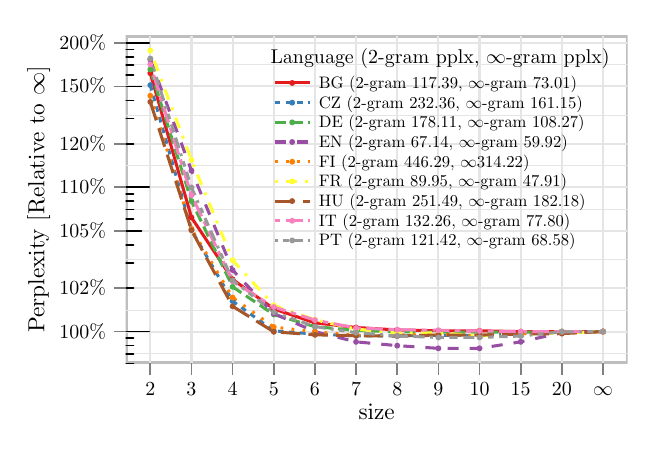
\begin{tikzpicture}[x=1pt,y=1pt]
\definecolor{fillColor}{RGB}{255,255,255}
\path[use as bounding box,fill=fillColor,fill opacity=0.00] (0,0) rectangle (216.81,144.54);
\begin{scope}
\path[clip] (  0.00,  0.00) rectangle (216.81,144.54);
\definecolor{fillColor}{RGB}{255,255,255}

\path[fill=fillColor] (  0.00,  0.00) rectangle (216.81,144.54);
\end{scope}
\begin{scope}
\path[clip] ( 35.40, 23.29) rectangle (216.81,141.69);
\definecolor{drawColor}{RGB}{190,190,190}

\path[draw=drawColor,line width= 1.5pt,line join=round,line cap=round] ( 35.40, 23.29) rectangle (216.81,141.69);
\definecolor{drawColor}{gray}{0.90}

\path[draw=drawColor,line width= 0.3pt,line join=round] ( 35.40, 26.85) --
	(216.81, 26.85);

\path[draw=drawColor,line width= 0.3pt,line join=round] ( 35.40, 42.55) --
	(216.81, 42.55);

\path[draw=drawColor,line width= 0.3pt,line join=round] ( 35.40, 60.78) --
	(216.81, 60.78);

\path[draw=drawColor,line width= 0.3pt,line join=round] ( 35.40, 79.01) --
	(216.81, 79.01);

\path[draw=drawColor,line width= 0.3pt,line join=round] ( 35.40, 94.71) --
	(216.81, 94.71);

\path[draw=drawColor,line width= 0.3pt,line join=round] ( 35.40,112.94) --
	(216.81,112.94);

\path[draw=drawColor,line width= 0.3pt,line join=round] ( 35.40,131.17) --
	(216.81,131.17);

\path[draw=drawColor,line width= 0.8pt,line join=round] ( 35.40, 34.70) --
	(216.81, 34.70);

\path[draw=drawColor,line width= 0.8pt,line join=round] ( 35.40, 50.40) --
	(216.81, 50.40);

\path[draw=drawColor,line width= 0.8pt,line join=round] ( 35.40, 71.16) --
	(216.81, 71.16);

\path[draw=drawColor,line width= 0.8pt,line join=round] ( 35.40, 86.86) --
	(216.81, 86.86);

\path[draw=drawColor,line width= 0.8pt,line join=round] ( 35.40,102.56) --
	(216.81,102.56);

\path[draw=drawColor,line width= 0.8pt,line join=round] ( 35.40,123.32) --
	(216.81,123.32);

\path[draw=drawColor,line width= 0.8pt,line join=round] ( 35.40,139.02) --
	(216.81,139.02);

\path[draw=drawColor,line width= 0.8pt,line join=round] ( 44.32, 23.29) --
	( 44.32,141.69);

\path[draw=drawColor,line width= 0.8pt,line join=round] ( 59.19, 23.29) --
	( 59.19,141.69);

\path[draw=drawColor,line width= 0.8pt,line join=round] ( 74.06, 23.29) --
	( 74.06,141.69);

\path[draw=drawColor,line width= 0.8pt,line join=round] ( 88.93, 23.29) --
	( 88.93,141.69);

\path[draw=drawColor,line width= 0.8pt,line join=round] (103.80, 23.29) --
	(103.80,141.69);

\path[draw=drawColor,line width= 0.8pt,line join=round] (118.67, 23.29) --
	(118.67,141.69);

\path[draw=drawColor,line width= 0.8pt,line join=round] (133.54, 23.29) --
	(133.54,141.69);

\path[draw=drawColor,line width= 0.8pt,line join=round] (148.41, 23.29) --
	(148.41,141.69);

\path[draw=drawColor,line width= 0.8pt,line join=round] (163.28, 23.29) --
	(163.28,141.69);

\path[draw=drawColor,line width= 0.8pt,line join=round] (178.15, 23.29) --
	(178.15,141.69);

\path[draw=drawColor,line width= 0.8pt,line join=round] (193.02, 23.29) --
	(193.02,141.69);

\path[draw=drawColor,line width= 0.8pt,line join=round] (207.89, 23.29) --
	(207.89,141.69);
\definecolor{drawColor}{RGB}{228,26,28}

\path[draw=drawColor,line width= 1.1pt,line join=round] ( 44.32,128.11) --
	( 59.19, 75.95) --
	( 74.06, 53.58) --
	( 88.93, 42.93) --
	(103.80, 37.88) --
	(118.67, 36.20) --
	(133.54, 35.31) --
	(148.41, 35.01) --
	(163.28, 35.01) --
	(178.15, 34.70) --
	(193.02, 34.70) --
	(207.89, 34.70);
\definecolor{drawColor}{RGB}{55,126,184}

\path[draw=drawColor,line width= 1.1pt,dash pattern=on 2pt off 2pt ,line join=round] ( 44.32,123.78) --
	( 59.19, 71.41) --
	( 74.06, 45.72) --
	( 88.93, 34.99) --
	(103.80, 33.81) --
	(118.67, 33.19) --
	(133.54, 33.19) --
	(148.41, 33.34) --
	(163.28, 33.34) --
	(178.15, 34.41) --
	(193.02, 34.55) --
	(207.89, 34.70);
\definecolor{drawColor}{RGB}{77,175,74}

\path[draw=drawColor,line width= 1.1pt,dash pattern=on 4pt off 2pt ,line join=round] ( 44.32,129.43) --
	( 59.19, 81.86) --
	( 74.06, 50.89) --
	( 88.93, 40.89) --
	(103.80, 36.51) --
	(118.67, 35.12) --
	(133.54, 34.70) --
	(148.41, 34.49) --
	(163.28, 34.49) --
	(178.15, 34.49) --
	(193.02, 34.70) --
	(207.89, 34.70);
\definecolor{drawColor}{RGB}{152,78,163}

\path[draw=drawColor,line width= 1.1pt,dash pattern=on 4pt off 4pt ,line join=round] ( 44.32,132.99) --
	( 59.19, 92.89) --
	( 74.06, 56.94) --
	( 88.93, 41.23) --
	(103.80, 34.70) --
	(118.67, 31.01) --
	(133.54, 29.64) --
	(148.41, 28.67) --
	(163.28, 28.67) --
	(178.15, 31.01) --
	(193.02, 34.32) --
	(207.89, 34.70);
\definecolor{drawColor}{RGB}{255,127,0}

\path[draw=drawColor,line width= 1.1pt,dash pattern=on 1pt off 3pt ,line join=round] ( 44.32,119.92) --
	( 59.19, 71.83) --
	( 74.06, 47.02) --
	( 88.93, 36.37) --
	(103.80, 34.63) --
	(118.67, 33.44) --
	(133.54, 33.52) --
	(148.41, 33.67) --
	(163.28, 33.29) --
	(178.15, 33.97) --
	(193.02, 34.48) --
	(207.89, 34.70);
\definecolor{drawColor}{RGB}{255,255,51}

\path[draw=drawColor,line width= 1.1pt,dash pattern=on 1pt off 3pt on 4pt off 3pt ,line join=round] ( 44.32,136.31) --
	( 59.19, 96.73) --
	( 74.06, 60.54) --
	( 88.93, 44.21) --
	(103.80, 38.99) --
	(118.67, 35.63) --
	(133.54, 34.22) --
	(148.41, 34.22) --
	(163.28, 33.24) --
	(178.15, 33.74) --
	(193.02, 34.22) --
	(207.89, 34.70);
\definecolor{drawColor}{RGB}{166,86,40}

\path[draw=drawColor,line width= 1.1pt,dash pattern=on 7pt off 3pt ,line join=round] ( 44.32,117.71) --
	( 59.19, 71.37) --
	( 74.06, 43.85) --
	( 88.93, 34.64) --
	(103.80, 33.55) --
	(118.67, 33.23) --
	(133.54, 33.12) --
	(148.41, 33.49) --
	(163.28, 33.45) --
	(178.15, 33.81) --
	(193.02, 33.99) --
	(207.89, 34.70);
\definecolor{drawColor}{RGB}{247,129,191}

\path[draw=drawColor,line width= 1.1pt,dash pattern=on 2pt off 2pt on 6pt off 2pt ,line join=round] ( 44.32,131.26) --
	( 59.19, 84.00) --
	( 74.06, 52.90) --
	( 88.93, 43.58) --
	(103.80, 38.87) --
	(118.67, 36.02) --
	(133.54, 35.40) --
	(148.41, 35.21) --
	(163.28, 34.95) --
	(178.15, 34.72) --
	(193.02, 34.69) --
	(207.89, 34.70);
\definecolor{drawColor}{gray}{0.60}

\path[draw=drawColor,line width= 1.1pt,dash pattern=on 1pt off 2pt on 2pt off 2pt on 3pt off 2pt on 4pt off 2pt ,line join=round] ( 44.32,133.40) --
	( 59.19, 86.79) --
	( 74.06, 53.23) --
	( 88.93, 41.73) --
	(103.80, 36.54) --
	(118.67, 34.31) --
	(133.54, 33.17) --
	(148.41, 32.59) --
	(163.28, 32.62) --
	(178.15, 33.11) --
	(193.02, 34.63) --
	(207.89, 34.70);
\definecolor{fillColor}{RGB}{228,26,28}

\path[fill=fillColor] ( 44.32,128.11) circle (  1.07);

\path[fill=fillColor] ( 59.19, 75.95) circle (  1.07);

\path[fill=fillColor] ( 74.06, 53.58) circle (  1.07);

\path[fill=fillColor] ( 88.93, 42.93) circle (  1.07);

\path[fill=fillColor] (103.80, 37.88) circle (  1.07);

\path[fill=fillColor] (118.67, 36.20) circle (  1.07);

\path[fill=fillColor] (133.54, 35.31) circle (  1.07);

\path[fill=fillColor] (148.41, 35.01) circle (  1.07);

\path[fill=fillColor] (163.28, 35.01) circle (  1.07);

\path[fill=fillColor] (178.15, 34.70) circle (  1.07);

\path[fill=fillColor] (193.02, 34.70) circle (  1.07);

\path[fill=fillColor] (207.89, 34.70) circle (  1.07);
\definecolor{fillColor}{RGB}{55,126,184}

\path[fill=fillColor] ( 44.32,123.78) circle (  1.07);

\path[fill=fillColor] ( 59.19, 71.41) circle (  1.07);

\path[fill=fillColor] ( 74.06, 45.72) circle (  1.07);

\path[fill=fillColor] ( 88.93, 34.99) circle (  1.07);

\path[fill=fillColor] (103.80, 33.81) circle (  1.07);

\path[fill=fillColor] (118.67, 33.19) circle (  1.07);

\path[fill=fillColor] (133.54, 33.19) circle (  1.07);

\path[fill=fillColor] (148.41, 33.34) circle (  1.07);

\path[fill=fillColor] (163.28, 33.34) circle (  1.07);

\path[fill=fillColor] (178.15, 34.41) circle (  1.07);

\path[fill=fillColor] (193.02, 34.55) circle (  1.07);

\path[fill=fillColor] (207.89, 34.70) circle (  1.07);
\definecolor{fillColor}{RGB}{77,175,74}

\path[fill=fillColor] ( 44.32,129.43) circle (  1.07);

\path[fill=fillColor] ( 59.19, 81.86) circle (  1.07);

\path[fill=fillColor] ( 74.06, 50.89) circle (  1.07);

\path[fill=fillColor] ( 88.93, 40.89) circle (  1.07);

\path[fill=fillColor] (103.80, 36.51) circle (  1.07);

\path[fill=fillColor] (118.67, 35.12) circle (  1.07);

\path[fill=fillColor] (133.54, 34.70) circle (  1.07);

\path[fill=fillColor] (148.41, 34.49) circle (  1.07);

\path[fill=fillColor] (163.28, 34.49) circle (  1.07);

\path[fill=fillColor] (178.15, 34.49) circle (  1.07);

\path[fill=fillColor] (193.02, 34.70) circle (  1.07);

\path[fill=fillColor] (207.89, 34.70) circle (  1.07);
\definecolor{fillColor}{RGB}{152,78,163}

\path[fill=fillColor] ( 44.32,132.99) circle (  1.07);

\path[fill=fillColor] ( 59.19, 92.89) circle (  1.07);

\path[fill=fillColor] ( 74.06, 56.94) circle (  1.07);

\path[fill=fillColor] ( 88.93, 41.23) circle (  1.07);

\path[fill=fillColor] (103.80, 34.70) circle (  1.07);

\path[fill=fillColor] (118.67, 31.01) circle (  1.07);

\path[fill=fillColor] (133.54, 29.64) circle (  1.07);

\path[fill=fillColor] (148.41, 28.67) circle (  1.07);

\path[fill=fillColor] (163.28, 28.67) circle (  1.07);

\path[fill=fillColor] (178.15, 31.01) circle (  1.07);

\path[fill=fillColor] (193.02, 34.32) circle (  1.07);

\path[fill=fillColor] (207.89, 34.70) circle (  1.07);
\definecolor{fillColor}{RGB}{255,127,0}

\path[fill=fillColor] ( 44.32,119.92) circle (  1.07);

\path[fill=fillColor] ( 59.19, 71.83) circle (  1.07);

\path[fill=fillColor] ( 74.06, 47.02) circle (  1.07);

\path[fill=fillColor] ( 88.93, 36.37) circle (  1.07);

\path[fill=fillColor] (103.80, 34.63) circle (  1.07);

\path[fill=fillColor] (118.67, 33.44) circle (  1.07);

\path[fill=fillColor] (133.54, 33.52) circle (  1.07);

\path[fill=fillColor] (148.41, 33.67) circle (  1.07);

\path[fill=fillColor] (163.28, 33.29) circle (  1.07);

\path[fill=fillColor] (178.15, 33.97) circle (  1.07);

\path[fill=fillColor] (193.02, 34.48) circle (  1.07);

\path[fill=fillColor] (207.89, 34.70) circle (  1.07);
\definecolor{fillColor}{RGB}{255,255,51}

\path[fill=fillColor] ( 44.32,136.31) circle (  1.07);

\path[fill=fillColor] ( 59.19, 96.73) circle (  1.07);

\path[fill=fillColor] ( 74.06, 60.54) circle (  1.07);

\path[fill=fillColor] ( 88.93, 44.21) circle (  1.07);

\path[fill=fillColor] (103.80, 38.99) circle (  1.07);

\path[fill=fillColor] (118.67, 35.63) circle (  1.07);

\path[fill=fillColor] (133.54, 34.22) circle (  1.07);

\path[fill=fillColor] (148.41, 34.22) circle (  1.07);

\path[fill=fillColor] (163.28, 33.24) circle (  1.07);

\path[fill=fillColor] (178.15, 33.74) circle (  1.07);

\path[fill=fillColor] (193.02, 34.22) circle (  1.07);

\path[fill=fillColor] (207.89, 34.70) circle (  1.07);
\definecolor{fillColor}{RGB}{166,86,40}

\path[fill=fillColor] ( 44.32,117.71) circle (  1.07);

\path[fill=fillColor] ( 59.19, 71.37) circle (  1.07);

\path[fill=fillColor] ( 74.06, 43.85) circle (  1.07);

\path[fill=fillColor] ( 88.93, 34.64) circle (  1.07);

\path[fill=fillColor] (103.80, 33.55) circle (  1.07);

\path[fill=fillColor] (118.67, 33.23) circle (  1.07);

\path[fill=fillColor] (133.54, 33.12) circle (  1.07);

\path[fill=fillColor] (148.41, 33.49) circle (  1.07);

\path[fill=fillColor] (163.28, 33.45) circle (  1.07);

\path[fill=fillColor] (178.15, 33.81) circle (  1.07);

\path[fill=fillColor] (193.02, 33.99) circle (  1.07);

\path[fill=fillColor] (207.89, 34.70) circle (  1.07);
\definecolor{fillColor}{RGB}{247,129,191}

\path[fill=fillColor] ( 44.32,131.26) circle (  1.07);

\path[fill=fillColor] ( 59.19, 84.00) circle (  1.07);

\path[fill=fillColor] ( 74.06, 52.90) circle (  1.07);

\path[fill=fillColor] ( 88.93, 43.58) circle (  1.07);

\path[fill=fillColor] (103.80, 38.87) circle (  1.07);

\path[fill=fillColor] (118.67, 36.02) circle (  1.07);

\path[fill=fillColor] (133.54, 35.40) circle (  1.07);

\path[fill=fillColor] (148.41, 35.21) circle (  1.07);

\path[fill=fillColor] (163.28, 34.95) circle (  1.07);

\path[fill=fillColor] (178.15, 34.72) circle (  1.07);

\path[fill=fillColor] (193.02, 34.69) circle (  1.07);

\path[fill=fillColor] (207.89, 34.70) circle (  1.07);
\definecolor{fillColor}{gray}{0.60}

\path[fill=fillColor] ( 44.32,133.40) circle (  1.07);

\path[fill=fillColor] ( 59.19, 86.79) circle (  1.07);

\path[fill=fillColor] ( 74.06, 53.23) circle (  1.07);

\path[fill=fillColor] ( 88.93, 41.73) circle (  1.07);

\path[fill=fillColor] (103.80, 36.54) circle (  1.07);

\path[fill=fillColor] (118.67, 34.31) circle (  1.07);

\path[fill=fillColor] (133.54, 33.17) circle (  1.07);

\path[fill=fillColor] (148.41, 32.59) circle (  1.07);

\path[fill=fillColor] (163.28, 32.62) circle (  1.07);

\path[fill=fillColor] (178.15, 33.11) circle (  1.07);

\path[fill=fillColor] (193.02, 34.63) circle (  1.07);

\path[fill=fillColor] (207.89, 34.70) circle (  1.07);
\definecolor{drawColor}{RGB}{0,0,0}

\path[draw=drawColor,line width= 0.6pt,line join=round,line cap=round] ( 35.40,  7.43) -- ( 38.25,  7.43);

\path[draw=drawColor,line width= 0.6pt,line join=round,line cap=round] ( 35.40, 13.95) -- ( 38.25, 13.95);

\path[draw=drawColor,line width= 0.6pt,line join=round,line cap=round] ( 35.40, 19.00) -- ( 41.09, 19.00);

\path[draw=drawColor,line width= 0.6pt,line join=round,line cap=round] ( 35.40, 23.13) -- ( 38.25, 23.13);

\path[draw=drawColor,line width= 0.6pt,line join=round,line cap=round] ( 35.40, 26.62) -- ( 38.25, 26.62);

\path[draw=drawColor,line width= 0.6pt,line join=round,line cap=round] ( 35.40, 29.65) -- ( 38.25, 29.65);

\path[draw=drawColor,line width= 0.6pt,line join=round,line cap=round] ( 35.40, 32.31) -- ( 38.25, 32.31);

\path[draw=drawColor,line width= 0.6pt,line join=round,line cap=round] ( 35.40, 34.70) -- ( 43.94, 34.70);

\path[draw=drawColor,line width= 0.6pt,line join=round,line cap=round] ( 35.40, 50.40) -- ( 38.25, 50.40);

\path[draw=drawColor,line width= 0.6pt,line join=round,line cap=round] ( 35.40, 59.59) -- ( 38.25, 59.59);

\path[draw=drawColor,line width= 0.6pt,line join=round,line cap=round] ( 35.40, 66.10) -- ( 38.25, 66.10);

\path[draw=drawColor,line width= 0.6pt,line join=round,line cap=round] ( 35.40, 71.16) -- ( 41.09, 71.16);

\path[draw=drawColor,line width= 0.6pt,line join=round,line cap=round] ( 35.40, 75.29) -- ( 38.25, 75.29);

\path[draw=drawColor,line width= 0.6pt,line join=round,line cap=round] ( 35.40, 78.78) -- ( 38.25, 78.78);

\path[draw=drawColor,line width= 0.6pt,line join=round,line cap=round] ( 35.40, 81.80) -- ( 38.25, 81.80);

\path[draw=drawColor,line width= 0.6pt,line join=round,line cap=round] ( 35.40, 84.47) -- ( 38.25, 84.47);

\path[draw=drawColor,line width= 0.6pt,line join=round,line cap=round] ( 35.40, 86.86) -- ( 43.94, 86.86);

\path[draw=drawColor,line width= 0.6pt,line join=round,line cap=round] ( 35.40,102.56) -- ( 38.25,102.56);

\path[draw=drawColor,line width= 0.6pt,line join=round,line cap=round] ( 35.40,111.74) -- ( 38.25,111.74);

\path[draw=drawColor,line width= 0.6pt,line join=round,line cap=round] ( 35.40,118.26) -- ( 38.25,118.26);

\path[draw=drawColor,line width= 0.6pt,line join=round,line cap=round] ( 35.40,123.32) -- ( 41.09,123.32);

\path[draw=drawColor,line width= 0.6pt,line join=round,line cap=round] ( 35.40,127.45) -- ( 38.25,127.45);

\path[draw=drawColor,line width= 0.6pt,line join=round,line cap=round] ( 35.40,130.94) -- ( 38.25,130.94);

\path[draw=drawColor,line width= 0.6pt,line join=round,line cap=round] ( 35.40,133.96) -- ( 38.25,133.96);

\path[draw=drawColor,line width= 0.6pt,line join=round,line cap=round] ( 35.40,136.63) -- ( 38.25,136.63);

\path[draw=drawColor,line width= 0.6pt,line join=round,line cap=round] ( 35.40,139.02) -- ( 43.94,139.02);
\end{scope}
\begin{scope}
\path[clip] (  0.00,  0.00) rectangle (216.81,144.54);
\definecolor{drawColor}{RGB}{0,0,0}

\node[text=drawColor,anchor=base east,inner sep=0pt, outer sep=0pt, scale=  0.72] at ( 28.29, 32.36) {100\%};

\node[text=drawColor,anchor=base east,inner sep=0pt, outer sep=0pt, scale=  0.72] at ( 28.29, 48.06) {102\%};

\node[text=drawColor,anchor=base east,inner sep=0pt, outer sep=0pt, scale=  0.72] at ( 28.29, 68.81) {105\%};

\node[text=drawColor,anchor=base east,inner sep=0pt, outer sep=0pt, scale=  0.72] at ( 28.29, 84.52) {110\%};

\node[text=drawColor,anchor=base east,inner sep=0pt, outer sep=0pt, scale=  0.72] at ( 28.29,100.22) {120\%};

\node[text=drawColor,anchor=base east,inner sep=0pt, outer sep=0pt, scale=  0.72] at ( 28.29,120.97) {150\%};

\node[text=drawColor,anchor=base east,inner sep=0pt, outer sep=0pt, scale=  0.72] at ( 28.29,136.67) {200\%};
\end{scope}
\begin{scope}
\path[clip] (  0.00,  0.00) rectangle (216.81,144.54);
\definecolor{drawColor}{gray}{0.50}

\path[draw=drawColor,line width= 0.6pt,line join=round] ( 31.13, 34.70) --
	( 35.40, 34.70);

\path[draw=drawColor,line width= 0.6pt,line join=round] ( 31.13, 50.40) --
	( 35.40, 50.40);

\path[draw=drawColor,line width= 0.6pt,line join=round] ( 31.13, 71.16) --
	( 35.40, 71.16);

\path[draw=drawColor,line width= 0.6pt,line join=round] ( 31.13, 86.86) --
	( 35.40, 86.86);

\path[draw=drawColor,line width= 0.6pt,line join=round] ( 31.13,102.56) --
	( 35.40,102.56);

\path[draw=drawColor,line width= 0.6pt,line join=round] ( 31.13,123.32) --
	( 35.40,123.32);

\path[draw=drawColor,line width= 0.6pt,line join=round] ( 31.13,139.02) --
	( 35.40,139.02);
\end{scope}
\begin{scope}
\path[clip] (  0.00,  0.00) rectangle (216.81,144.54);
\definecolor{drawColor}{gray}{0.50}

\path[draw=drawColor,line width= 0.6pt,line join=round] ( 44.32, 19.02) --
	( 44.32, 23.29);

\path[draw=drawColor,line width= 0.6pt,line join=round] ( 59.19, 19.02) --
	( 59.19, 23.29);

\path[draw=drawColor,line width= 0.6pt,line join=round] ( 74.06, 19.02) --
	( 74.06, 23.29);

\path[draw=drawColor,line width= 0.6pt,line join=round] ( 88.93, 19.02) --
	( 88.93, 23.29);

\path[draw=drawColor,line width= 0.6pt,line join=round] (103.80, 19.02) --
	(103.80, 23.29);

\path[draw=drawColor,line width= 0.6pt,line join=round] (118.67, 19.02) --
	(118.67, 23.29);

\path[draw=drawColor,line width= 0.6pt,line join=round] (133.54, 19.02) --
	(133.54, 23.29);

\path[draw=drawColor,line width= 0.6pt,line join=round] (148.41, 19.02) --
	(148.41, 23.29);

\path[draw=drawColor,line width= 0.6pt,line join=round] (163.28, 19.02) --
	(163.28, 23.29);

\path[draw=drawColor,line width= 0.6pt,line join=round] (178.15, 19.02) --
	(178.15, 23.29);

\path[draw=drawColor,line width= 0.6pt,line join=round] (193.02, 19.02) --
	(193.02, 23.29);

\path[draw=drawColor,line width= 0.6pt,line join=round] (207.89, 19.02) --
	(207.89, 23.29);
\end{scope}
\begin{scope}
\path[clip] (  0.00,  0.00) rectangle (216.81,144.54);
\definecolor{drawColor}{RGB}{0,0,0}

\node[text=drawColor,anchor=base,inner sep=0pt, outer sep=0pt, scale=  0.72] at ( 44.32, 11.49) {2};

\node[text=drawColor,anchor=base,inner sep=0pt, outer sep=0pt, scale=  0.72] at ( 59.19, 11.49) {3};

\node[text=drawColor,anchor=base,inner sep=0pt, outer sep=0pt, scale=  0.72] at ( 74.06, 11.49) {4};

\node[text=drawColor,anchor=base,inner sep=0pt, outer sep=0pt, scale=  0.72] at ( 88.93, 11.49) {5};

\node[text=drawColor,anchor=base,inner sep=0pt, outer sep=0pt, scale=  0.72] at (103.80, 11.49) {6};

\node[text=drawColor,anchor=base,inner sep=0pt, outer sep=0pt, scale=  0.72] at (118.67, 11.49) {7};

\node[text=drawColor,anchor=base,inner sep=0pt, outer sep=0pt, scale=  0.72] at (133.54, 11.49) {8};

\node[text=drawColor,anchor=base,inner sep=0pt, outer sep=0pt, scale=  0.72] at (148.41, 11.49) {9};

\node[text=drawColor,anchor=base,inner sep=0pt, outer sep=0pt, scale=  0.72] at (163.28, 11.49) {10};

\node[text=drawColor,anchor=base,inner sep=0pt, outer sep=0pt, scale=  0.72] at (178.15, 11.49) {15};

\node[text=drawColor,anchor=base,inner sep=0pt, outer sep=0pt, scale=  0.72] at (193.02, 11.49) {20};

\node[text=drawColor,anchor=base,inner sep=0pt, outer sep=0pt, scale=  0.72] at (207.89, 11.49) {$\infty$};
\end{scope}
\begin{scope}
\path[clip] (  0.00,  0.00) rectangle (216.81,144.54);
\definecolor{drawColor}{RGB}{0,0,0}

\node[text=drawColor,anchor=base,inner sep=0pt, outer sep=0pt, scale=  0.84] at (126.11,  3.01) {\ngram size};
\end{scope}
\begin{scope}
\path[clip] (  0.00,  0.00) rectangle (216.81,144.54);
\definecolor{drawColor}{RGB}{0,0,0}

\node[text=drawColor,rotate= 90.00,anchor=base,inner sep=0pt, outer sep=0pt, scale=  0.84] at (  6.07, 82.49) {Perplexity [Relative to $\infty$]};
\end{scope}
\begin{scope}
\path[clip] (  0.00,  0.00) rectangle (216.81,144.54);
\definecolor{drawColor}{RGB}{0,0,0}

\node[text=drawColor,anchor=base west,inner sep=0pt, outer sep=0pt, scale=  0.72] at ( 87.76,131.73) {Language ($2$-gram pplx, $\infty$-gram pplx)};
\end{scope}
\begin{scope}
\path[clip] (  0.00,  0.00) rectangle (216.81,144.54);
\definecolor{drawColor}{RGB}{228,26,28}

\path[draw=drawColor,line width= 1.1pt,line join=round] ( 89.32,124.56) -- (101.84,124.56);
\end{scope}
\begin{scope}
\path[clip] (  0.00,  0.00) rectangle (216.81,144.54);
\definecolor{fillColor}{RGB}{228,26,28}

\path[fill=fillColor] ( 95.58,124.56) circle (  1.07);
\end{scope}
\begin{scope}
\path[clip] (  0.00,  0.00) rectangle (216.81,144.54);
\definecolor{drawColor}{RGB}{55,126,184}

\path[draw=drawColor,line width= 1.1pt,dash pattern=on 2pt off 2pt ,line join=round] ( 89.32,117.44) -- (101.84,117.44);
\end{scope}
\begin{scope}
\path[clip] (  0.00,  0.00) rectangle (216.81,144.54);
\definecolor{fillColor}{RGB}{55,126,184}

\path[fill=fillColor] ( 95.58,117.44) circle (  1.07);
\end{scope}
\begin{scope}
\path[clip] (  0.00,  0.00) rectangle (216.81,144.54);
\definecolor{drawColor}{RGB}{77,175,74}

\path[draw=drawColor,line width= 1.1pt,dash pattern=on 4pt off 2pt ,line join=round] ( 89.32,110.33) -- (101.84,110.33);
\end{scope}
\begin{scope}
\path[clip] (  0.00,  0.00) rectangle (216.81,144.54);
\definecolor{fillColor}{RGB}{77,175,74}

\path[fill=fillColor] ( 95.58,110.33) circle (  1.07);
\end{scope}
\begin{scope}
\path[clip] (  0.00,  0.00) rectangle (216.81,144.54);
\definecolor{drawColor}{RGB}{152,78,163}

\path[draw=drawColor,line width= 1.1pt,dash pattern=on 4pt off 4pt ,line join=round] ( 89.32,103.22) -- (101.84,103.22);
\end{scope}
\begin{scope}
\path[clip] (  0.00,  0.00) rectangle (216.81,144.54);
\definecolor{fillColor}{RGB}{152,78,163}

\path[fill=fillColor] ( 95.58,103.22) circle (  1.07);
\end{scope}
\begin{scope}
\path[clip] (  0.00,  0.00) rectangle (216.81,144.54);
\definecolor{drawColor}{RGB}{255,127,0}

\path[draw=drawColor,line width= 1.1pt,dash pattern=on 1pt off 3pt ,line join=round] ( 89.32, 96.10) -- (101.84, 96.10);
\end{scope}
\begin{scope}
\path[clip] (  0.00,  0.00) rectangle (216.81,144.54);
\definecolor{fillColor}{RGB}{255,127,0}

\path[fill=fillColor] ( 95.58, 96.10) circle (  1.07);
\end{scope}
\begin{scope}
\path[clip] (  0.00,  0.00) rectangle (216.81,144.54);
\definecolor{drawColor}{RGB}{255,255,51}

\path[draw=drawColor,line width= 1.1pt,dash pattern=on 1pt off 3pt on 4pt off 3pt ,line join=round] ( 89.32, 88.99) -- (101.84, 88.99);
\end{scope}
\begin{scope}
\path[clip] (  0.00,  0.00) rectangle (216.81,144.54);
\definecolor{fillColor}{RGB}{255,255,51}

\path[fill=fillColor] ( 95.58, 88.99) circle (  1.07);
\end{scope}
\begin{scope}
\path[clip] (  0.00,  0.00) rectangle (216.81,144.54);
\definecolor{drawColor}{RGB}{166,86,40}

\path[draw=drawColor,line width= 1.1pt,dash pattern=on 7pt off 3pt ,line join=round] ( 89.32, 81.88) -- (101.84, 81.88);
\end{scope}
\begin{scope}
\path[clip] (  0.00,  0.00) rectangle (216.81,144.54);
\definecolor{fillColor}{RGB}{166,86,40}

\path[fill=fillColor] ( 95.58, 81.88) circle (  1.07);
\end{scope}
\begin{scope}
\path[clip] (  0.00,  0.00) rectangle (216.81,144.54);
\definecolor{drawColor}{RGB}{247,129,191}

\path[draw=drawColor,line width= 1.1pt,dash pattern=on 2pt off 2pt on 6pt off 2pt ,line join=round] ( 89.32, 74.76) -- (101.84, 74.76);
\end{scope}
\begin{scope}
\path[clip] (  0.00,  0.00) rectangle (216.81,144.54);
\definecolor{fillColor}{RGB}{247,129,191}

\path[fill=fillColor] ( 95.58, 74.76) circle (  1.07);
\end{scope}
\begin{scope}
\path[clip] (  0.00,  0.00) rectangle (216.81,144.54);
\definecolor{drawColor}{gray}{0.60}

\path[draw=drawColor,line width= 1.1pt,dash pattern=on 1pt off 2pt on 2pt off 2pt on 3pt off 2pt on 4pt off 2pt ,line join=round] ( 89.32, 67.65) -- (101.84, 67.65);
\end{scope}
\begin{scope}
\path[clip] (  0.00,  0.00) rectangle (216.81,144.54);
\definecolor{fillColor}{gray}{0.60}

\path[fill=fillColor] ( 95.58, 67.65) circle (  1.07);
\end{scope}
\begin{scope}
\path[clip] (  0.00,  0.00) rectangle (216.81,144.54);
\definecolor{drawColor}{RGB}{0,0,0}

\node[text=drawColor,anchor=base west,inner sep=0pt, outer sep=0pt, scale=  0.60] at (105.22,122.60) {BG ($2$-gram $117.39$, $\infty$-gram $73.01$)};
\end{scope}
\begin{scope}
\path[clip] (  0.00,  0.00) rectangle (216.81,144.54);
\definecolor{drawColor}{RGB}{0,0,0}

\node[text=drawColor,anchor=base west,inner sep=0pt, outer sep=0pt, scale=  0.60] at (105.22,115.49) {CZ ($2$-gram $232.36$, $\infty$-gram $161.15$)};
\end{scope}
\begin{scope}
\path[clip] (  0.00,  0.00) rectangle (216.81,144.54);
\definecolor{drawColor}{RGB}{0,0,0}

\node[text=drawColor,anchor=base west,inner sep=0pt, outer sep=0pt, scale=  0.60] at (105.22,108.38) {DE ($2$-gram $178.11$, $\infty$-gram $108.27$)};
\end{scope}
\begin{scope}
\path[clip] (  0.00,  0.00) rectangle (216.81,144.54);
\definecolor{drawColor}{RGB}{0,0,0}

\node[text=drawColor,anchor=base west,inner sep=0pt, outer sep=0pt, scale=  0.60] at (105.22,101.26) {EN ($2$-gram $67.14$, $\infty$-gram $59.92$)};
\end{scope}
\begin{scope}
\path[clip] (  0.00,  0.00) rectangle (216.81,144.54);
\definecolor{drawColor}{RGB}{0,0,0}

\node[text=drawColor,anchor=base west,inner sep=0pt, outer sep=0pt, scale=  0.60] at (105.22, 94.15) {FI ($2$-gram $446.29$, $\infty 314.22$)};
\end{scope}
\begin{scope}
\path[clip] (  0.00,  0.00) rectangle (216.81,144.54);
\definecolor{drawColor}{RGB}{0,0,0}

\node[text=drawColor,anchor=base west,inner sep=0pt, outer sep=0pt, scale=  0.60] at (105.22, 87.04) {FR ($2$-gram $89.95$, $\infty$-gram $47.91$)};
\end{scope}
\begin{scope}
\path[clip] (  0.00,  0.00) rectangle (216.81,144.54);
\definecolor{drawColor}{RGB}{0,0,0}

\node[text=drawColor,anchor=base west,inner sep=0pt, outer sep=0pt, scale=  0.60] at (105.22, 79.92) {HU ($2$-gram $251.49$, $\infty$-gram $182.18$)};
\end{scope}
\begin{scope}
\path[clip] (  0.00,  0.00) rectangle (216.81,144.54);
\definecolor{drawColor}{RGB}{0,0,0}

\node[text=drawColor,anchor=base west,inner sep=0pt, outer sep=0pt, scale=  0.60] at (105.22, 72.81) {IT ($2$-gram $132.26$, $\infty$-gram $77.80$)};
\end{scope}
\begin{scope}
\path[clip] (  0.00,  0.00) rectangle (216.81,144.54);
\definecolor{drawColor}{RGB}{0,0,0}

\node[text=drawColor,anchor=base west,inner sep=0pt, outer sep=0pt, scale=  0.60] at (105.22, 65.70) {PT ($2$-gram $121.42$, $\infty$-gram $68.58$)};
\end{scope}
\end{tikzpicture}

\caption{Perplexity results on several Europarl languages for different \ngram sizes, $m=2\ldots10,15,20,\infty$.}
\label{fig:pplx}
\end{figure}

%\paragraph{Perplexity}
We evaluated the perplexity across different languages and using \ngrams of varying order from $m=2$ to $\infty$ (unbounded), as shown on Figure~\ref{fig:pplx}.
Our results matched the perplexity results from \SRILM (for smaller values of $m$ in which \SRILM training was feasible, $m \le 10$).
Note that perplexity drops dramatically from $m=2\ldots5$ however the gains thereafter are modest for most languages.
Despite this, several large \ngram matches were found
 %as illustrated                               in Figure~\ref{fig:germanpattern}, 
ranging in size up to a $34$-gram match.
We speculate that the perplexity plateau is due to the simplistic Kneser-Ney discounting formula which is not designed for higher order \ngram LMs and appear to discount large \ngrams too aggressively. 
We leave further exploration of richer discounting techniques such as Modified Kneser-Ney \cite{chen1996empirical} or the Sequence Memoizer \cite{wood2011sequence} to our future work.





% \begin{figure}[tb]
% 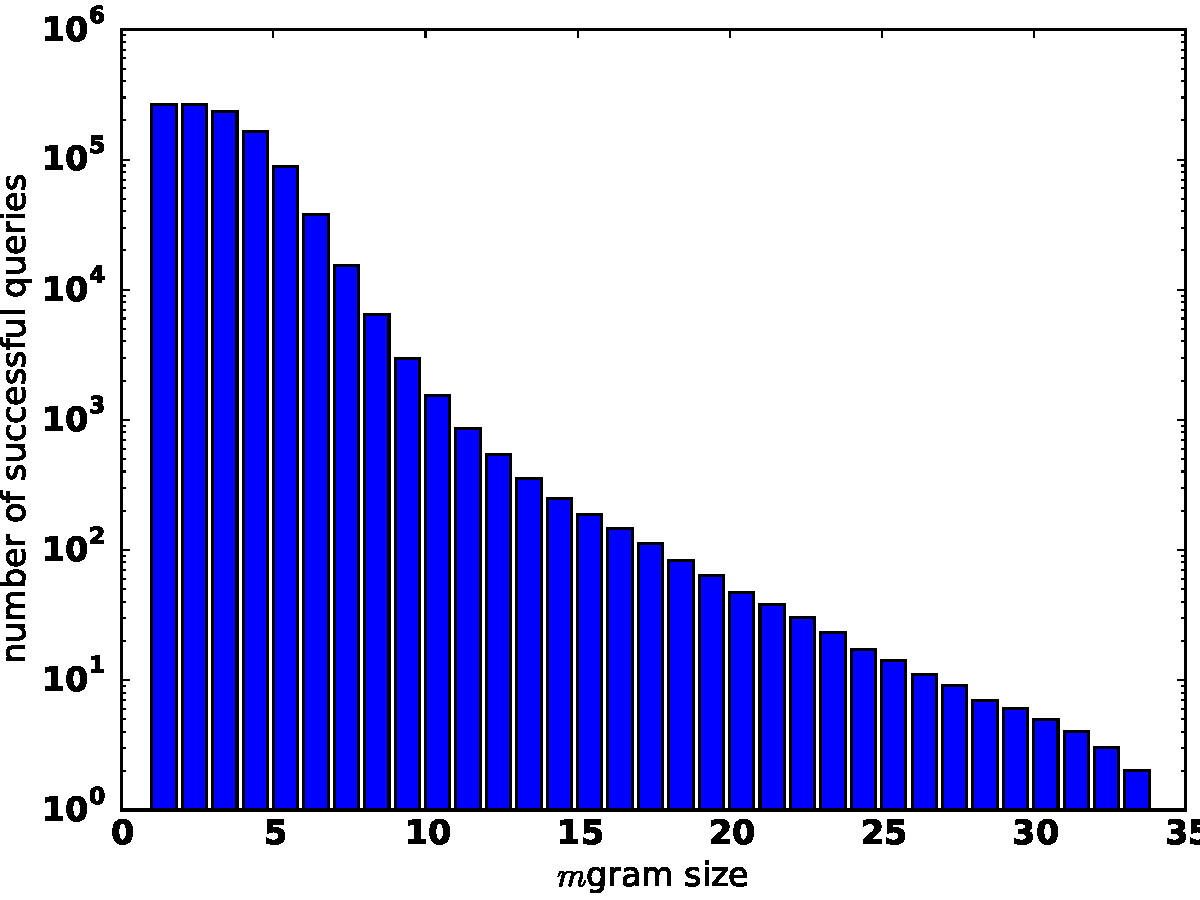
\includegraphics[width=\columnwidth]{figures/german_pattern_size.pdf}
% \caption{Number of \ngrams of different sizes in both training and test sets for Europarl German}
% %\caption{Number of successful queries across different pattern sizes from KN computation over the German test set, with unbounded $m$.}
% \label{fig:germanpattern}
% \end{figure}


%\paragraph{Time vs.\ Space}
Figure~\ref{fig:spacetime} compares space and time of our indexes with \SRILM on the German part of Europarl.
The construction cost of our indexes in terms of both space and time is comparable to that of 
a $3/4$-gram \SRILM\ index. The space usage of \dualCST\ index is comparable to
a compact $3$-gram \SRILM\ index. Our \singleCST\ index uses only \mb{177} RAM
at query time, which is comparable to the size of the collection (\mb{172}).
However, query processing is significantly slower for both our structures.
For $2$-grams, \dualCST\ is $3$ times slower than a $2$-gram \SRILM\ index as
the expensive $\nlplus{\dotpatdot}$ is not computed. However, for large \ngrams,
our indexes are much slower than \SRILM. For $m>2$, 
the \dualCST\ index is roughly six times slower than \singleCST. Our fastest
index, is $10$ times slower than the slowest \SRILM $10$-gram index. However,
our run-time is independent of $\plen$. Thus, as $m$ increases, our index
will become more competitive to \SRILM\ while using a constant amount of space.


\begin{figure}[tb]
% Created by tikzDevice version 0.8.1 on 2015-05-31 14:38:55
% !TEX encoding = UTF-8 Unicode
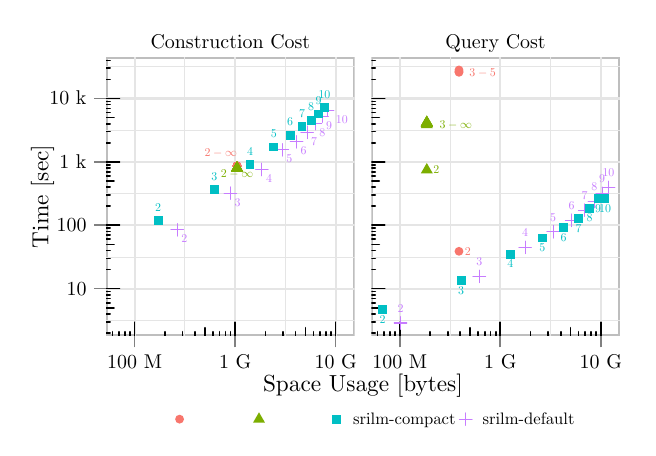
\begin{tikzpicture}[x=1pt,y=1pt]
\definecolor{fillColor}{RGB}{255,255,255}
\path[use as bounding box,fill=fillColor,fill opacity=0.00] (0,0) rectangle (216.81,144.54);
\begin{scope}
\path[clip] (  0.00,  0.00) rectangle (216.81,144.54);
\definecolor{fillColor}{RGB}{255,255,255}

\path[fill=fillColor] (  0.00,  0.00) rectangle (216.81,144.54);
\end{scope}
\begin{scope}
\path[clip] ( 28.36,133.83) rectangle (118.15,144.54);

\path[] ( 28.36,133.83) rectangle (118.15,144.54);
\definecolor{drawColor}{RGB}{0,0,0}

\node[text=drawColor,anchor=base,inner sep=0pt, outer sep=0pt, scale=  0.72] at ( 73.25,136.84) {Construction Cost};
\end{scope}
\begin{scope}
\path[clip] (124.17,133.83) rectangle (213.96,144.54);

\path[] (124.17,133.83) rectangle (213.96,144.54);
\definecolor{drawColor}{RGB}{0,0,0}

\node[text=drawColor,anchor=base,inner sep=0pt, outer sep=0pt, scale=  0.72] at (169.07,136.84) {Query Cost};
\end{scope}
\begin{scope}
\path[clip] ( 28.36, 33.25) rectangle (118.15,133.83);
\definecolor{drawColor}{RGB}{190,190,190}

\path[draw=drawColor,line width= 1.5pt,line join=round,line cap=round] ( 28.36, 33.25) rectangle (118.15,133.83);
\definecolor{drawColor}{gray}{0.90}

\path[draw=drawColor,line width= 0.3pt,line join=round] ( 28.36, 38.79) --
	(118.15, 38.79);

\path[draw=drawColor,line width= 0.3pt,line join=round] ( 28.36, 61.69) --
	(118.15, 61.69);

\path[draw=drawColor,line width= 0.3pt,line join=round] ( 28.36, 84.59) --
	(118.15, 84.59);

\path[draw=drawColor,line width= 0.3pt,line join=round] ( 28.36,107.49) --
	(118.15,107.49);

\path[draw=drawColor,line width= 0.3pt,line join=round] ( 28.36,130.39) --
	(118.15,130.39);

\path[draw=drawColor,line width= 0.3pt,line join=round] ( 56.81, 33.25) --
	( 56.81,133.83);

\path[draw=drawColor,line width= 0.3pt,line join=round] ( 93.13, 33.25) --
	( 93.13,133.83);

\path[draw=drawColor,line width= 0.8pt,line join=round] ( 28.36, 50.24) --
	(118.15, 50.24);

\path[draw=drawColor,line width= 0.8pt,line join=round] ( 28.36, 73.14) --
	(118.15, 73.14);

\path[draw=drawColor,line width= 0.8pt,line join=round] ( 28.36, 96.04) --
	(118.15, 96.04);

\path[draw=drawColor,line width= 0.8pt,line join=round] ( 28.36,118.94) --
	(118.15,118.94);

\path[draw=drawColor,line width= 0.8pt,line join=round] ( 38.65, 33.25) --
	( 38.65,133.83);

\path[draw=drawColor,line width= 0.8pt,line join=round] ( 74.97, 33.25) --
	( 74.97,133.83);

\path[draw=drawColor,line width= 0.8pt,line join=round] (111.29, 33.25) --
	(111.29,133.83);
\definecolor{drawColor}{RGB}{0,0,0}

\path[draw=drawColor,line width= 0.6pt,line join=round,line cap=round] (  2.34, 33.25) -- (  2.34, 38.09);

\path[draw=drawColor,line width= 0.6pt,line join=round,line cap=round] ( 13.27, 33.25) -- ( 13.27, 34.67);

\path[draw=drawColor,line width= 0.6pt,line join=round,line cap=round] ( 19.67, 33.25) -- ( 19.67, 34.67);

\path[draw=drawColor,line width= 0.6pt,line join=round,line cap=round] ( 24.20, 33.25) -- ( 24.20, 34.67);

\path[draw=drawColor,line width= 0.6pt,line join=round,line cap=round] ( 27.72, 33.25) -- ( 27.72, 36.09);

\path[draw=drawColor,line width= 0.6pt,line join=round,line cap=round] ( 30.60, 33.25) -- ( 30.60, 34.67);

\path[draw=drawColor,line width= 0.6pt,line join=round,line cap=round] ( 33.03, 33.25) -- ( 33.03, 34.67);

\path[draw=drawColor,line width= 0.6pt,line join=round,line cap=round] ( 35.14, 33.25) -- ( 35.14, 34.67);

\path[draw=drawColor,line width= 0.6pt,line join=round,line cap=round] ( 36.99, 33.25) -- ( 36.99, 34.67);

\path[draw=drawColor,line width= 0.6pt,line join=round,line cap=round] ( 38.65, 33.25) -- ( 38.65, 38.09);

\path[draw=drawColor,line width= 0.6pt,line join=round,line cap=round] ( 49.59, 33.25) -- ( 49.59, 34.67);

\path[draw=drawColor,line width= 0.6pt,line join=round,line cap=round] ( 55.98, 33.25) -- ( 55.98, 34.67);

\path[draw=drawColor,line width= 0.6pt,line join=round,line cap=round] ( 60.52, 33.25) -- ( 60.52, 34.67);

\path[draw=drawColor,line width= 0.6pt,line join=round,line cap=round] ( 64.04, 33.25) -- ( 64.04, 36.09);

\path[draw=drawColor,line width= 0.6pt,line join=round,line cap=round] ( 66.91, 33.25) -- ( 66.91, 34.67);

\path[draw=drawColor,line width= 0.6pt,line join=round,line cap=round] ( 69.34, 33.25) -- ( 69.34, 34.67);

\path[draw=drawColor,line width= 0.6pt,line join=round,line cap=round] ( 71.45, 33.25) -- ( 71.45, 34.67);

\path[draw=drawColor,line width= 0.6pt,line join=round,line cap=round] ( 73.31, 33.25) -- ( 73.31, 34.67);

\path[draw=drawColor,line width= 0.6pt,line join=round,line cap=round] ( 74.97, 33.25) -- ( 74.97, 38.09);

\path[draw=drawColor,line width= 0.6pt,line join=round,line cap=round] ( 85.90, 33.25) -- ( 85.90, 34.67);

\path[draw=drawColor,line width= 0.6pt,line join=round,line cap=round] ( 92.30, 33.25) -- ( 92.30, 34.67);

\path[draw=drawColor,line width= 0.6pt,line join=round,line cap=round] ( 96.83, 33.25) -- ( 96.83, 34.67);

\path[draw=drawColor,line width= 0.6pt,line join=round,line cap=round] (100.35, 33.25) -- (100.35, 36.09);

\path[draw=drawColor,line width= 0.6pt,line join=round,line cap=round] (103.23, 33.25) -- (103.23, 34.67);

\path[draw=drawColor,line width= 0.6pt,line join=round,line cap=round] (105.66, 33.25) -- (105.66, 34.67);

\path[draw=drawColor,line width= 0.6pt,line join=round,line cap=round] (107.77, 33.25) -- (107.77, 34.67);

\path[draw=drawColor,line width= 0.6pt,line join=round,line cap=round] (109.62, 33.25) -- (109.62, 34.67);

\path[draw=drawColor,line width= 0.6pt,line join=round,line cap=round] (111.29, 33.25) -- (111.29, 38.09);

\path[draw=drawColor,line width= 0.6pt,line join=round,line cap=round] (122.22, 33.25) -- (122.22, 34.67);

\path[draw=drawColor,line width= 0.6pt,line join=round,line cap=round] (128.61, 33.25) -- (128.61, 34.67);

\path[draw=drawColor,line width= 0.6pt,line join=round,line cap=round] (133.15, 33.25) -- (133.15, 34.67);

\path[draw=drawColor,line width= 0.6pt,line join=round,line cap=round] (136.67, 33.25) -- (136.67, 36.09);

\path[draw=drawColor,line width= 0.6pt,line join=round,line cap=round] (139.54, 33.25) -- (139.54, 34.67);

\path[draw=drawColor,line width= 0.6pt,line join=round,line cap=round] (141.98, 33.25) -- (141.98, 34.67);

\path[draw=drawColor,line width= 0.6pt,line join=round,line cap=round] (144.08, 33.25) -- (144.08, 34.67);

\path[draw=drawColor,line width= 0.6pt,line join=round,line cap=round] (145.94, 33.25) -- (145.94, 34.67);

\path[draw=drawColor,line width= 0.6pt,line join=round,line cap=round] (147.60, 33.25) -- (147.60, 38.09);

\path[draw=drawColor,line width= 0.6pt,line join=round,line cap=round] ( 28.36, 27.34) -- ( 33.20, 27.34);

\path[draw=drawColor,line width= 0.6pt,line join=round,line cap=round] ( 28.36, 34.23) -- ( 29.78, 34.23);

\path[draw=drawColor,line width= 0.6pt,line join=round,line cap=round] ( 28.36, 38.26) -- ( 29.78, 38.26);

\path[draw=drawColor,line width= 0.6pt,line join=round,line cap=round] ( 28.36, 41.12) -- ( 29.78, 41.12);

\path[draw=drawColor,line width= 0.6pt,line join=round,line cap=round] ( 28.36, 43.34) -- ( 31.20, 43.34);

\path[draw=drawColor,line width= 0.6pt,line join=round,line cap=round] ( 28.36, 45.16) -- ( 29.78, 45.16);

\path[draw=drawColor,line width= 0.6pt,line join=round,line cap=round] ( 28.36, 46.69) -- ( 29.78, 46.69);

\path[draw=drawColor,line width= 0.6pt,line join=round,line cap=round] ( 28.36, 48.02) -- ( 29.78, 48.02);

\path[draw=drawColor,line width= 0.6pt,line join=round,line cap=round] ( 28.36, 49.19) -- ( 29.78, 49.19);

\path[draw=drawColor,line width= 0.6pt,line join=round,line cap=round] ( 28.36, 50.24) -- ( 33.20, 50.24);

\path[draw=drawColor,line width= 0.6pt,line join=round,line cap=round] ( 28.36, 57.13) -- ( 29.78, 57.13);

\path[draw=drawColor,line width= 0.6pt,line join=round,line cap=round] ( 28.36, 61.16) -- ( 29.78, 61.16);

\path[draw=drawColor,line width= 0.6pt,line join=round,line cap=round] ( 28.36, 64.02) -- ( 29.78, 64.02);

\path[draw=drawColor,line width= 0.6pt,line join=round,line cap=round] ( 28.36, 66.24) -- ( 31.20, 66.24);

\path[draw=drawColor,line width= 0.6pt,line join=round,line cap=round] ( 28.36, 68.06) -- ( 29.78, 68.06);

\path[draw=drawColor,line width= 0.6pt,line join=round,line cap=round] ( 28.36, 69.59) -- ( 29.78, 69.59);

\path[draw=drawColor,line width= 0.6pt,line join=round,line cap=round] ( 28.36, 70.92) -- ( 29.78, 70.92);

\path[draw=drawColor,line width= 0.6pt,line join=round,line cap=round] ( 28.36, 72.09) -- ( 29.78, 72.09);

\path[draw=drawColor,line width= 0.6pt,line join=round,line cap=round] ( 28.36, 73.14) -- ( 33.20, 73.14);

\path[draw=drawColor,line width= 0.6pt,line join=round,line cap=round] ( 28.36, 80.03) -- ( 29.78, 80.03);

\path[draw=drawColor,line width= 0.6pt,line join=round,line cap=round] ( 28.36, 84.07) -- ( 29.78, 84.07);

\path[draw=drawColor,line width= 0.6pt,line join=round,line cap=round] ( 28.36, 86.93) -- ( 29.78, 86.93);

\path[draw=drawColor,line width= 0.6pt,line join=round,line cap=round] ( 28.36, 89.15) -- ( 31.20, 89.15);

\path[draw=drawColor,line width= 0.6pt,line join=round,line cap=round] ( 28.36, 90.96) -- ( 29.78, 90.96);

\path[draw=drawColor,line width= 0.6pt,line join=round,line cap=round] ( 28.36, 92.49) -- ( 29.78, 92.49);

\path[draw=drawColor,line width= 0.6pt,line join=round,line cap=round] ( 28.36, 93.82) -- ( 29.78, 93.82);

\path[draw=drawColor,line width= 0.6pt,line join=round,line cap=round] ( 28.36, 94.99) -- ( 29.78, 94.99);

\path[draw=drawColor,line width= 0.6pt,line join=round,line cap=round] ( 28.36, 96.04) -- ( 33.20, 96.04);

\path[draw=drawColor,line width= 0.6pt,line join=round,line cap=round] ( 28.36,102.93) -- ( 29.78,102.93);

\path[draw=drawColor,line width= 0.6pt,line join=round,line cap=round] ( 28.36,106.97) -- ( 29.78,106.97);

\path[draw=drawColor,line width= 0.6pt,line join=round,line cap=round] ( 28.36,109.83) -- ( 29.78,109.83);

\path[draw=drawColor,line width= 0.6pt,line join=round,line cap=round] ( 28.36,112.05) -- ( 31.20,112.05);

\path[draw=drawColor,line width= 0.6pt,line join=round,line cap=round] ( 28.36,113.86) -- ( 29.78,113.86);

\path[draw=drawColor,line width= 0.6pt,line join=round,line cap=round] ( 28.36,115.39) -- ( 29.78,115.39);

\path[draw=drawColor,line width= 0.6pt,line join=round,line cap=round] ( 28.36,116.72) -- ( 29.78,116.72);

\path[draw=drawColor,line width= 0.6pt,line join=round,line cap=round] ( 28.36,117.89) -- ( 29.78,117.89);

\path[draw=drawColor,line width= 0.6pt,line join=round,line cap=round] ( 28.36,118.94) -- ( 33.20,118.94);

\path[draw=drawColor,line width= 0.6pt,line join=round,line cap=round] ( 28.36,125.84) -- ( 29.78,125.84);

\path[draw=drawColor,line width= 0.6pt,line join=round,line cap=round] ( 28.36,129.87) -- ( 29.78,129.87);

\path[draw=drawColor,line width= 0.6pt,line join=round,line cap=round] ( 28.36,132.73) -- ( 29.78,132.73);

\path[draw=drawColor,line width= 0.6pt,line join=round,line cap=round] ( 28.36,134.95) -- ( 31.20,134.95);

\path[draw=drawColor,line width= 0.6pt,line join=round,line cap=round] ( 28.36,136.76) -- ( 29.78,136.76);

\path[draw=drawColor,line width= 0.6pt,line join=round,line cap=round] ( 28.36,138.30) -- ( 29.78,138.30);

\path[draw=drawColor,line width= 0.6pt,line join=round,line cap=round] ( 28.36,139.62) -- ( 29.78,139.62);

\path[draw=drawColor,line width= 0.6pt,line join=round,line cap=round] ( 28.36,140.80) -- ( 29.78,140.80);

\path[draw=drawColor,line width= 0.6pt,line join=round,line cap=round] ( 28.36,141.84) -- ( 33.20,141.84);
\definecolor{drawColor}{RGB}{199,124,255}

\path[draw=drawColor,line width= 0.4pt,line join=round,line cap=round] ( 51.78, 71.49) -- ( 56.30, 71.49);

\path[draw=drawColor,line width= 0.4pt,line join=round,line cap=round] ( 54.04, 69.23) -- ( 54.04, 73.75);

\path[draw=drawColor,line width= 0.4pt,line join=round,line cap=round] ( 71.01, 84.73) -- ( 75.53, 84.73);

\path[draw=drawColor,line width= 0.4pt,line join=round,line cap=round] ( 73.27, 82.47) -- ( 73.27, 86.99);

\path[draw=drawColor,line width= 0.4pt,line join=round,line cap=round] ( 82.38, 93.31) -- ( 86.91, 93.31);

\path[draw=drawColor,line width= 0.4pt,line join=round,line cap=round] ( 84.65, 91.04) -- ( 84.65, 95.57);

\path[draw=drawColor,line width= 0.4pt,line join=round,line cap=round] ( 89.76,100.37) -- ( 94.28,100.37);

\path[draw=drawColor,line width= 0.4pt,line join=round,line cap=round] ( 92.02, 98.11) -- ( 92.02,102.64);

\path[draw=drawColor,line width= 0.4pt,line join=round,line cap=round] ( 94.89,103.29) -- ( 99.41,103.29);

\path[draw=drawColor,line width= 0.4pt,line join=round,line cap=round] ( 97.15,101.03) -- ( 97.15,105.55);

\path[draw=drawColor,line width= 0.4pt,line join=round,line cap=round] ( 98.71,106.75) -- (103.24,106.75);

\path[draw=drawColor,line width= 0.4pt,line join=round,line cap=round] (100.98,104.49) -- (100.98,109.01);

\path[draw=drawColor,line width= 0.4pt,line join=round,line cap=round] (101.70,109.84) -- (106.23,109.84);

\path[draw=drawColor,line width= 0.4pt,line join=round,line cap=round] (103.96,107.58) -- (103.96,112.10);

\path[draw=drawColor,line width= 0.4pt,line join=round,line cap=round] (104.12,112.58) -- (108.64,112.58);

\path[draw=drawColor,line width= 0.4pt,line join=round,line cap=round] (106.38,110.32) -- (106.38,114.85);

\path[draw=drawColor,line width= 0.4pt,line join=round,line cap=round] (106.12,114.77) -- (110.65,114.77);

\path[draw=drawColor,line width= 0.4pt,line join=round,line cap=round] (108.38,112.51) -- (108.38,117.04);
\definecolor{fillColor}{RGB}{0,191,196}

\path[fill=fillColor] ( 45.55, 73.26) --
	( 48.75, 73.26) --
	( 48.75, 76.46) --
	( 45.55, 76.46) --
	cycle;

\path[fill=fillColor] ( 65.83, 84.45) --
	( 69.03, 84.45) --
	( 69.03, 87.65) --
	( 65.83, 87.65) --
	cycle;

\path[fill=fillColor] ( 78.75, 93.45) --
	( 81.96, 93.45) --
	( 81.96, 96.65) --
	( 78.75, 96.65) --
	cycle;

\path[fill=fillColor] ( 87.33, 99.84) --
	( 90.53, 99.84) --
	( 90.53,103.04) --
	( 87.33,103.04) --
	cycle;

\path[fill=fillColor] ( 93.24,104.12) --
	( 96.44,104.12) --
	( 96.44,107.33) --
	( 93.24,107.33) --
	cycle;

\path[fill=fillColor] ( 97.55,107.25) --
	(100.75,107.25) --
	(100.75,110.45) --
	( 97.55,110.45) --
	cycle;

\path[fill=fillColor] (100.86,109.53) --
	(104.06,109.53) --
	(104.06,112.74) --
	(100.86,112.74) --
	cycle;

\path[fill=fillColor] (103.49,111.77) --
	(106.69,111.77) --
	(106.69,114.97) --
	(103.49,114.97) --
	cycle;

\path[fill=fillColor] (105.65,114.08) --
	(108.85,114.08) --
	(108.85,117.28) --
	(105.65,117.28) --
	cycle;
\definecolor{fillColor}{RGB}{248,118,109}

\path[fill=fillColor] ( 75.65, 94.55) circle (  1.60);

\path[fill=fillColor] ( 75.65, 94.55) circle (  1.60);

\path[fill=fillColor] ( 75.65, 94.55) circle (  1.60);

\path[fill=fillColor] ( 75.65, 94.55) circle (  1.60);

\path[fill=fillColor] ( 75.65, 94.55) circle (  1.60);

\path[fill=fillColor] ( 75.65, 94.55) circle (  1.60);

\path[fill=fillColor] ( 75.65, 94.55) circle (  1.60);

\path[fill=fillColor] ( 75.65, 94.55) circle (  1.60);

\path[fill=fillColor] ( 75.65, 94.55) circle (  1.60);
\definecolor{fillColor}{RGB}{124,174,0}

\path[fill=fillColor] ( 75.65, 96.27) --
	( 77.81, 92.54) --
	( 73.50, 92.54) --
	cycle;

\path[fill=fillColor] ( 75.65, 96.27) --
	( 77.81, 92.54) --
	( 73.50, 92.54) --
	cycle;

\path[fill=fillColor] ( 75.65, 96.27) --
	( 77.81, 92.54) --
	( 73.50, 92.54) --
	cycle;

\path[fill=fillColor] ( 75.65, 96.27) --
	( 77.81, 92.54) --
	( 73.50, 92.54) --
	cycle;

\path[fill=fillColor] ( 75.65, 96.27) --
	( 77.81, 92.54) --
	( 73.50, 92.54) --
	cycle;

\path[fill=fillColor] ( 75.65, 96.27) --
	( 77.81, 92.54) --
	( 73.50, 92.54) --
	cycle;

\path[fill=fillColor] ( 75.65, 96.27) --
	( 77.81, 92.54) --
	( 73.50, 92.54) --
	cycle;

\path[fill=fillColor] ( 75.65, 96.27) --
	( 77.81, 92.54) --
	( 73.50, 92.54) --
	cycle;

\path[fill=fillColor] ( 75.65, 96.27) --
	( 77.81, 92.54) --
	( 73.50, 92.54) --
	cycle;

\node[text=drawColor,anchor=base west,inner sep=0pt, outer sep=0pt, scale=  0.43] at ( 55.53, 66.78) {2};

\node[text=drawColor,anchor=base west,inner sep=0pt, outer sep=0pt, scale=  0.43] at ( 74.76, 80.02) {3};

\node[text=drawColor,anchor=base west,inner sep=0pt, outer sep=0pt, scale=  0.43] at ( 86.13, 88.60) {4};

\node[text=drawColor,anchor=base west,inner sep=0pt, outer sep=0pt, scale=  0.43] at ( 93.51, 95.67) {5};

\node[text=drawColor,anchor=base west,inner sep=0pt, outer sep=0pt, scale=  0.43] at ( 98.64, 98.58) {6};

\node[text=drawColor,anchor=base west,inner sep=0pt, outer sep=0pt, scale=  0.43] at (102.46,102.04) {7};

\node[text=drawColor,anchor=base west,inner sep=0pt, outer sep=0pt, scale=  0.43] at (105.45,105.14) {8};

\node[text=drawColor,anchor=base west,inner sep=0pt, outer sep=0pt, scale=  0.43] at (107.87,107.88) {9};

\node[text=drawColor,anchor=base west,inner sep=0pt, outer sep=0pt, scale=  0.43] at (111.36,110.07) {10};
\definecolor{drawColor}{RGB}{0,191,196}

\node[text=drawColor,anchor=base,inner sep=0pt, outer sep=0pt, scale=  0.43] at ( 47.15, 78.18) {2};

\node[text=drawColor,anchor=base,inner sep=0pt, outer sep=0pt, scale=  0.43] at ( 67.43, 89.38) {3};

\node[text=drawColor,anchor=base,inner sep=0pt, outer sep=0pt, scale=  0.43] at ( 80.35, 98.37) {4};

\node[text=drawColor,anchor=base,inner sep=0pt, outer sep=0pt, scale=  0.43] at ( 88.93,104.76) {5};

\node[text=drawColor,anchor=base,inner sep=0pt, outer sep=0pt, scale=  0.43] at ( 94.84,109.05) {6};

\node[text=drawColor,anchor=base,inner sep=0pt, outer sep=0pt, scale=  0.43] at ( 99.15,112.17) {7};

\node[text=drawColor,anchor=base,inner sep=0pt, outer sep=0pt, scale=  0.43] at (102.46,114.46) {8};

\node[text=drawColor,anchor=base,inner sep=0pt, outer sep=0pt, scale=  0.43] at (105.09,116.69) {9};

\node[text=drawColor,anchor=base,inner sep=0pt, outer sep=0pt, scale=  0.43] at (107.25,119.00) {10};
\definecolor{drawColor}{RGB}{248,118,109}

\node[text=drawColor,anchor=base east,inner sep=0pt, outer sep=0pt, scale=  0.43] at ( 75.65, 97.87) {$2-\\\infty$};
\definecolor{drawColor}{RGB}{124,174,0}

\node[text=drawColor,anchor=base,inner sep=0pt, outer sep=0pt, scale=  0.43] at ( 75.65, 90.46) {$2-\\\infty$};
\end{scope}
\begin{scope}
\path[clip] (124.17, 33.25) rectangle (213.96,133.83);
\definecolor{drawColor}{RGB}{190,190,190}

\path[draw=drawColor,line width= 1.5pt,line join=round,line cap=round] (124.17, 33.25) rectangle (213.96,133.83);
\definecolor{drawColor}{gray}{0.90}

\path[draw=drawColor,line width= 0.3pt,line join=round] (124.17, 38.79) --
	(213.96, 38.79);

\path[draw=drawColor,line width= 0.3pt,line join=round] (124.17, 61.69) --
	(213.96, 61.69);

\path[draw=drawColor,line width= 0.3pt,line join=round] (124.17, 84.59) --
	(213.96, 84.59);

\path[draw=drawColor,line width= 0.3pt,line join=round] (124.17,107.49) --
	(213.96,107.49);

\path[draw=drawColor,line width= 0.3pt,line join=round] (124.17,130.39) --
	(213.96,130.39);

\path[draw=drawColor,line width= 0.3pt,line join=round] (152.63, 33.25) --
	(152.63,133.83);

\path[draw=drawColor,line width= 0.3pt,line join=round] (188.94, 33.25) --
	(188.94,133.83);

\path[draw=drawColor,line width= 0.8pt,line join=round] (124.17, 50.24) --
	(213.96, 50.24);

\path[draw=drawColor,line width= 0.8pt,line join=round] (124.17, 73.14) --
	(213.96, 73.14);

\path[draw=drawColor,line width= 0.8pt,line join=round] (124.17, 96.04) --
	(213.96, 96.04);

\path[draw=drawColor,line width= 0.8pt,line join=round] (124.17,118.94) --
	(213.96,118.94);

\path[draw=drawColor,line width= 0.8pt,line join=round] (134.47, 33.25) --
	(134.47,133.83);

\path[draw=drawColor,line width= 0.8pt,line join=round] (170.78, 33.25) --
	(170.78,133.83);

\path[draw=drawColor,line width= 0.8pt,line join=round] (207.10, 33.25) --
	(207.10,133.83);
\definecolor{drawColor}{RGB}{0,0,0}

\path[draw=drawColor,line width= 0.6pt,line join=round,line cap=round] ( 98.15, 33.25) -- ( 98.15, 38.09);

\path[draw=drawColor,line width= 0.6pt,line join=round,line cap=round] (109.09, 33.25) -- (109.09, 34.67);

\path[draw=drawColor,line width= 0.6pt,line join=round,line cap=round] (115.48, 33.25) -- (115.48, 34.67);

\path[draw=drawColor,line width= 0.6pt,line join=round,line cap=round] (120.02, 33.25) -- (120.02, 34.67);

\path[draw=drawColor,line width= 0.6pt,line join=round,line cap=round] (123.54, 33.25) -- (123.54, 36.09);

\path[draw=drawColor,line width= 0.6pt,line join=round,line cap=round] (126.41, 33.25) -- (126.41, 34.67);

\path[draw=drawColor,line width= 0.6pt,line join=round,line cap=round] (128.84, 33.25) -- (128.84, 34.67);

\path[draw=drawColor,line width= 0.6pt,line join=round,line cap=round] (130.95, 33.25) -- (130.95, 34.67);

\path[draw=drawColor,line width= 0.6pt,line join=round,line cap=round] (132.81, 33.25) -- (132.81, 34.67);

\path[draw=drawColor,line width= 0.6pt,line join=round,line cap=round] (134.47, 33.25) -- (134.47, 38.09);

\path[draw=drawColor,line width= 0.6pt,line join=round,line cap=round] (145.40, 33.25) -- (145.40, 34.67);

\path[draw=drawColor,line width= 0.6pt,line join=round,line cap=round] (151.80, 33.25) -- (151.80, 34.67);

\path[draw=drawColor,line width= 0.6pt,line join=round,line cap=round] (156.33, 33.25) -- (156.33, 34.67);

\path[draw=drawColor,line width= 0.6pt,line join=round,line cap=round] (159.85, 33.25) -- (159.85, 36.09);

\path[draw=drawColor,line width= 0.6pt,line join=round,line cap=round] (162.73, 33.25) -- (162.73, 34.67);

\path[draw=drawColor,line width= 0.6pt,line join=round,line cap=round] (165.16, 33.25) -- (165.16, 34.67);

\path[draw=drawColor,line width= 0.6pt,line join=round,line cap=round] (167.26, 33.25) -- (167.26, 34.67);

\path[draw=drawColor,line width= 0.6pt,line join=round,line cap=round] (169.12, 33.25) -- (169.12, 34.67);

\path[draw=drawColor,line width= 0.6pt,line join=round,line cap=round] (170.78, 33.25) -- (170.78, 38.09);

\path[draw=drawColor,line width= 0.6pt,line join=round,line cap=round] (181.72, 33.25) -- (181.72, 34.67);

\path[draw=drawColor,line width= 0.6pt,line join=round,line cap=round] (188.11, 33.25) -- (188.11, 34.67);

\path[draw=drawColor,line width= 0.6pt,line join=round,line cap=round] (192.65, 33.25) -- (192.65, 34.67);

\path[draw=drawColor,line width= 0.6pt,line join=round,line cap=round] (196.17, 33.25) -- (196.17, 36.09);

\path[draw=drawColor,line width= 0.6pt,line join=round,line cap=round] (199.04, 33.25) -- (199.04, 34.67);

\path[draw=drawColor,line width= 0.6pt,line join=round,line cap=round] (201.47, 33.25) -- (201.47, 34.67);

\path[draw=drawColor,line width= 0.6pt,line join=round,line cap=round] (203.58, 33.25) -- (203.58, 34.67);

\path[draw=drawColor,line width= 0.6pt,line join=round,line cap=round] (205.44, 33.25) -- (205.44, 34.67);

\path[draw=drawColor,line width= 0.6pt,line join=round,line cap=round] (207.10, 33.25) -- (207.10, 38.09);

\path[draw=drawColor,line width= 0.6pt,line join=round,line cap=round] (124.17, 27.34) -- (129.01, 27.34);

\path[draw=drawColor,line width= 0.6pt,line join=round,line cap=round] (124.17, 34.23) -- (125.60, 34.23);

\path[draw=drawColor,line width= 0.6pt,line join=round,line cap=round] (124.17, 38.26) -- (125.60, 38.26);

\path[draw=drawColor,line width= 0.6pt,line join=round,line cap=round] (124.17, 41.12) -- (125.60, 41.12);

\path[draw=drawColor,line width= 0.6pt,line join=round,line cap=round] (124.17, 43.34) -- (127.02, 43.34);

\path[draw=drawColor,line width= 0.6pt,line join=round,line cap=round] (124.17, 45.16) -- (125.60, 45.16);

\path[draw=drawColor,line width= 0.6pt,line join=round,line cap=round] (124.17, 46.69) -- (125.60, 46.69);

\path[draw=drawColor,line width= 0.6pt,line join=round,line cap=round] (124.17, 48.02) -- (125.60, 48.02);

\path[draw=drawColor,line width= 0.6pt,line join=round,line cap=round] (124.17, 49.19) -- (125.60, 49.19);

\path[draw=drawColor,line width= 0.6pt,line join=round,line cap=round] (124.17, 50.24) -- (129.01, 50.24);

\path[draw=drawColor,line width= 0.6pt,line join=round,line cap=round] (124.17, 57.13) -- (125.60, 57.13);

\path[draw=drawColor,line width= 0.6pt,line join=round,line cap=round] (124.17, 61.16) -- (125.60, 61.16);

\path[draw=drawColor,line width= 0.6pt,line join=round,line cap=round] (124.17, 64.02) -- (125.60, 64.02);

\path[draw=drawColor,line width= 0.6pt,line join=round,line cap=round] (124.17, 66.24) -- (127.02, 66.24);

\path[draw=drawColor,line width= 0.6pt,line join=round,line cap=round] (124.17, 68.06) -- (125.60, 68.06);

\path[draw=drawColor,line width= 0.6pt,line join=round,line cap=round] (124.17, 69.59) -- (125.60, 69.59);

\path[draw=drawColor,line width= 0.6pt,line join=round,line cap=round] (124.17, 70.92) -- (125.60, 70.92);

\path[draw=drawColor,line width= 0.6pt,line join=round,line cap=round] (124.17, 72.09) -- (125.60, 72.09);

\path[draw=drawColor,line width= 0.6pt,line join=round,line cap=round] (124.17, 73.14) -- (129.01, 73.14);

\path[draw=drawColor,line width= 0.6pt,line join=round,line cap=round] (124.17, 80.03) -- (125.60, 80.03);

\path[draw=drawColor,line width= 0.6pt,line join=round,line cap=round] (124.17, 84.07) -- (125.60, 84.07);

\path[draw=drawColor,line width= 0.6pt,line join=round,line cap=round] (124.17, 86.93) -- (125.60, 86.93);

\path[draw=drawColor,line width= 0.6pt,line join=round,line cap=round] (124.17, 89.15) -- (127.02, 89.15);

\path[draw=drawColor,line width= 0.6pt,line join=round,line cap=round] (124.17, 90.96) -- (125.60, 90.96);

\path[draw=drawColor,line width= 0.6pt,line join=round,line cap=round] (124.17, 92.49) -- (125.60, 92.49);

\path[draw=drawColor,line width= 0.6pt,line join=round,line cap=round] (124.17, 93.82) -- (125.60, 93.82);

\path[draw=drawColor,line width= 0.6pt,line join=round,line cap=round] (124.17, 94.99) -- (125.60, 94.99);

\path[draw=drawColor,line width= 0.6pt,line join=round,line cap=round] (124.17, 96.04) -- (129.01, 96.04);

\path[draw=drawColor,line width= 0.6pt,line join=round,line cap=round] (124.17,102.93) -- (125.60,102.93);

\path[draw=drawColor,line width= 0.6pt,line join=round,line cap=round] (124.17,106.97) -- (125.60,106.97);

\path[draw=drawColor,line width= 0.6pt,line join=round,line cap=round] (124.17,109.83) -- (125.60,109.83);

\path[draw=drawColor,line width= 0.6pt,line join=round,line cap=round] (124.17,112.05) -- (127.02,112.05);

\path[draw=drawColor,line width= 0.6pt,line join=round,line cap=round] (124.17,113.86) -- (125.60,113.86);

\path[draw=drawColor,line width= 0.6pt,line join=round,line cap=round] (124.17,115.39) -- (125.60,115.39);

\path[draw=drawColor,line width= 0.6pt,line join=round,line cap=round] (124.17,116.72) -- (125.60,116.72);

\path[draw=drawColor,line width= 0.6pt,line join=round,line cap=round] (124.17,117.89) -- (125.60,117.89);

\path[draw=drawColor,line width= 0.6pt,line join=round,line cap=round] (124.17,118.94) -- (129.01,118.94);

\path[draw=drawColor,line width= 0.6pt,line join=round,line cap=round] (124.17,125.84) -- (125.60,125.84);

\path[draw=drawColor,line width= 0.6pt,line join=round,line cap=round] (124.17,129.87) -- (125.60,129.87);

\path[draw=drawColor,line width= 0.6pt,line join=round,line cap=round] (124.17,132.73) -- (125.60,132.73);

\path[draw=drawColor,line width= 0.6pt,line join=round,line cap=round] (124.17,134.95) -- (127.02,134.95);

\path[draw=drawColor,line width= 0.6pt,line join=round,line cap=round] (124.17,136.76) -- (125.60,136.76);

\path[draw=drawColor,line width= 0.6pt,line join=round,line cap=round] (124.17,138.30) -- (125.60,138.30);

\path[draw=drawColor,line width= 0.6pt,line join=round,line cap=round] (124.17,139.62) -- (125.60,139.62);

\path[draw=drawColor,line width= 0.6pt,line join=round,line cap=round] (124.17,140.80) -- (125.60,140.80);

\path[draw=drawColor,line width= 0.6pt,line join=round,line cap=round] (124.17,141.84) -- (129.01,141.84);
\definecolor{drawColor}{RGB}{199,124,255}

\path[draw=drawColor,line width= 0.4pt,line join=round,line cap=round] (132.47, 37.82) -- (136.99, 37.82);

\path[draw=drawColor,line width= 0.4pt,line join=round,line cap=round] (134.73, 35.56) -- (134.73, 40.08);

\path[draw=drawColor,line width= 0.4pt,line join=round,line cap=round] (160.92, 54.66) -- (165.45, 54.66);

\path[draw=drawColor,line width= 0.4pt,line join=round,line cap=round] (163.18, 52.40) -- (163.18, 56.92);

\path[draw=drawColor,line width= 0.4pt,line join=round,line cap=round] (177.49, 65.14) -- (182.01, 65.14);

\path[draw=drawColor,line width= 0.4pt,line join=round,line cap=round] (179.75, 62.88) -- (179.75, 67.41);

\path[draw=drawColor,line width= 0.4pt,line join=round,line cap=round] (187.63, 70.80) -- (192.15, 70.80);

\path[draw=drawColor,line width= 0.4pt,line join=round,line cap=round] (189.89, 68.53) -- (189.89, 73.06);

\path[draw=drawColor,line width= 0.4pt,line join=round,line cap=round] (194.27, 74.94) -- (198.80, 74.94);

\path[draw=drawColor,line width= 0.4pt,line join=round,line cap=round] (196.54, 72.67) -- (196.54, 77.20);

\path[draw=drawColor,line width= 0.4pt,line join=round,line cap=round] (198.98, 78.59) -- (203.51, 78.59);

\path[draw=drawColor,line width= 0.4pt,line join=round,line cap=round] (201.24, 76.33) -- (201.24, 80.85);

\path[draw=drawColor,line width= 0.4pt,line join=round,line cap=round] (202.53, 81.70) -- (207.06, 81.70);

\path[draw=drawColor,line width= 0.4pt,line join=round,line cap=round] (204.80, 79.44) -- (204.80, 83.96);

\path[draw=drawColor,line width= 0.4pt,line join=round,line cap=round] (205.34, 84.67) -- (209.86, 84.67);

\path[draw=drawColor,line width= 0.4pt,line join=round,line cap=round] (207.60, 82.40) -- (207.60, 86.93);

\path[draw=drawColor,line width= 0.4pt,line join=round,line cap=round] (207.62, 86.78) -- (212.15, 86.78);

\path[draw=drawColor,line width= 0.4pt,line join=round,line cap=round] (209.88, 84.52) -- (209.88, 89.04);
\definecolor{fillColor}{RGB}{0,191,196}

\path[fill=fillColor] (126.65, 41.06) --
	(129.85, 41.06) --
	(129.85, 44.26) --
	(126.65, 44.26) --
	cycle;

\path[fill=fillColor] (155.05, 51.52) --
	(158.25, 51.52) --
	(158.25, 54.72) --
	(155.05, 54.72) --
	cycle;

\path[fill=fillColor] (172.79, 61.12) --
	(175.99, 61.12) --
	(175.99, 64.32) --
	(172.79, 64.32) --
	cycle;

\path[fill=fillColor] (184.34, 66.93) --
	(187.54, 66.93) --
	(187.54, 70.13) --
	(184.34, 70.13) --
	cycle;

\path[fill=fillColor] (192.06, 70.71) --
	(195.26, 70.71) --
	(195.26, 73.91) --
	(192.06, 73.91) --
	cycle;

\path[fill=fillColor] (197.46, 73.83) --
	(200.66, 73.83) --
	(200.66, 77.03) --
	(197.46, 77.03) --
	cycle;

\path[fill=fillColor] (201.45, 77.75) --
	(204.65, 77.75) --
	(204.65, 80.95) --
	(201.45, 80.95) --
	cycle;

\path[fill=fillColor] (204.55, 81.21) --
	(207.75, 81.21) --
	(207.75, 84.41) --
	(204.55, 84.41) --
	cycle;

\path[fill=fillColor] (207.03, 81.07) --
	(210.23, 81.07) --
	(210.23, 84.27) --
	(207.03, 84.27) --
	cycle;
\definecolor{fillColor}{RGB}{248,118,109}

\path[fill=fillColor] (155.85, 63.73) circle (  1.60);

\path[fill=fillColor] (155.85,128.41) circle (  1.60);

\path[fill=fillColor] (155.85,128.63) circle (  1.60);

\path[fill=fillColor] (155.85,129.26) circle (  1.60);
\definecolor{fillColor}{RGB}{124,174,0}

\path[fill=fillColor] (144.22, 95.64) --
	(146.38, 91.91) --
	(142.07, 91.91) --
	cycle;

\path[fill=fillColor] (144.22,111.98) --
	(146.38,108.25) --
	(142.07,108.25) --
	cycle;

\path[fill=fillColor] (144.22,112.64) --
	(146.38,108.91) --
	(142.07,108.91) --
	cycle;

\path[fill=fillColor] (144.22,112.42) --
	(146.38,108.69) --
	(142.07,108.69) --
	cycle;

\path[fill=fillColor] (144.22,112.47) --
	(146.38,108.73) --
	(142.07,108.73) --
	cycle;

\path[fill=fillColor] (144.22,112.80) --
	(146.38,109.06) --
	(142.07,109.06) --
	cycle;

\path[fill=fillColor] (144.22,112.63) --
	(146.38,108.90) --
	(142.07,108.90) --
	cycle;

\path[fill=fillColor] (144.22,112.83) --
	(146.38,109.09) --
	(142.07,109.09) --
	cycle;

\path[fill=fillColor] (144.22,112.59) --
	(146.38,108.85) --
	(142.07,108.85) --
	cycle;
\definecolor{drawColor}{RGB}{248,118,109}

\node[text=drawColor,anchor=base west,inner sep=0pt, outer sep=0pt, scale=  0.43] at (157.98, 62.35) {$2$};

\node[text=drawColor,anchor=base west,inner sep=0pt, outer sep=0pt, scale=  0.43] at (159.63,127.03) {$3-5$};
\definecolor{drawColor}{RGB}{124,174,0}

\node[text=drawColor,anchor=base west,inner sep=0pt, outer sep=0pt, scale=  0.43] at (146.56, 91.77) {$2$};

\node[text=drawColor,anchor=base west,inner sep=0pt, outer sep=0pt, scale=  0.43] at (148.85,108.11) {$3-\\\infty$};
\definecolor{drawColor}{RGB}{199,124,255}

\node[text=drawColor,anchor=base,inner sep=0pt, outer sep=0pt, scale=  0.43] at (134.73, 41.70) {2};

\node[text=drawColor,anchor=base,inner sep=0pt, outer sep=0pt, scale=  0.43] at (163.18, 58.53) {3};

\node[text=drawColor,anchor=base,inner sep=0pt, outer sep=0pt, scale=  0.43] at (179.75, 69.02) {4};

\node[text=drawColor,anchor=base,inner sep=0pt, outer sep=0pt, scale=  0.43] at (189.89, 74.67) {5};

\node[text=drawColor,anchor=base,inner sep=0pt, outer sep=0pt, scale=  0.43] at (196.54, 78.81) {6};

\node[text=drawColor,anchor=base,inner sep=0pt, outer sep=0pt, scale=  0.43] at (201.24, 82.47) {7};

\node[text=drawColor,anchor=base,inner sep=0pt, outer sep=0pt, scale=  0.43] at (204.80, 85.57) {8};

\node[text=drawColor,anchor=base,inner sep=0pt, outer sep=0pt, scale=  0.43] at (207.60, 88.54) {9};

\node[text=drawColor,anchor=base,inner sep=0pt, outer sep=0pt, scale=  0.43] at (209.88, 90.66) {10};
\definecolor{drawColor}{RGB}{0,191,196}

\node[text=drawColor,anchor=base,inner sep=0pt, outer sep=0pt, scale=  0.43] at (128.25, 37.68) {2};

\node[text=drawColor,anchor=base,inner sep=0pt, outer sep=0pt, scale=  0.43] at (156.65, 48.13) {3};

\node[text=drawColor,anchor=base,inner sep=0pt, outer sep=0pt, scale=  0.43] at (174.39, 57.73) {4};

\node[text=drawColor,anchor=base,inner sep=0pt, outer sep=0pt, scale=  0.43] at (185.94, 63.55) {5};

\node[text=drawColor,anchor=base,inner sep=0pt, outer sep=0pt, scale=  0.43] at (193.66, 67.33) {6};

\node[text=drawColor,anchor=base,inner sep=0pt, outer sep=0pt, scale=  0.43] at (199.06, 70.45) {7};

\node[text=drawColor,anchor=base,inner sep=0pt, outer sep=0pt, scale=  0.43] at (203.05, 74.37) {8};

\node[text=drawColor,anchor=base,inner sep=0pt, outer sep=0pt, scale=  0.43] at (206.15, 77.83) {9};

\node[text=drawColor,anchor=base,inner sep=0pt, outer sep=0pt, scale=  0.43] at (208.63, 77.68) {10};
\end{scope}
\begin{scope}
\path[clip] (  0.00,  0.00) rectangle (216.81,144.54);
\definecolor{drawColor}{RGB}{0,0,0}

\node[text=drawColor,anchor=base east,inner sep=0pt, outer sep=0pt, scale=  0.72] at ( 21.25, 47.89) {10};

\node[text=drawColor,anchor=base east,inner sep=0pt, outer sep=0pt, scale=  0.72] at ( 21.25, 70.79) {100};

\node[text=drawColor,anchor=base east,inner sep=0pt, outer sep=0pt, scale=  0.72] at ( 21.25, 93.70) {1 k};

\node[text=drawColor,anchor=base east,inner sep=0pt, outer sep=0pt, scale=  0.72] at ( 21.25,116.60) {10 k};
\end{scope}
\begin{scope}
\path[clip] (  0.00,  0.00) rectangle (216.81,144.54);
\definecolor{drawColor}{gray}{0.50}

\path[draw=drawColor,line width= 0.6pt,line join=round] ( 24.09, 50.24) --
	( 28.36, 50.24);

\path[draw=drawColor,line width= 0.6pt,line join=round] ( 24.09, 73.14) --
	( 28.36, 73.14);

\path[draw=drawColor,line width= 0.6pt,line join=round] ( 24.09, 96.04) --
	( 28.36, 96.04);

\path[draw=drawColor,line width= 0.6pt,line join=round] ( 24.09,118.94) --
	( 28.36,118.94);
\end{scope}
\begin{scope}
\path[clip] (  0.00,  0.00) rectangle (216.81,144.54);
\definecolor{drawColor}{gray}{0.50}

\path[draw=drawColor,line width= 0.6pt,line join=round] ( 38.65, 28.98) --
	( 38.65, 33.25);

\path[draw=drawColor,line width= 0.6pt,line join=round] ( 74.97, 28.98) --
	( 74.97, 33.25);

\path[draw=drawColor,line width= 0.6pt,line join=round] (111.29, 28.98) --
	(111.29, 33.25);
\end{scope}
\begin{scope}
\path[clip] (  0.00,  0.00) rectangle (216.81,144.54);
\definecolor{drawColor}{RGB}{0,0,0}

\node[text=drawColor,anchor=base,inner sep=0pt, outer sep=0pt, scale=  0.72] at ( 38.65, 21.45) {100 M};

\node[text=drawColor,anchor=base,inner sep=0pt, outer sep=0pt, scale=  0.72] at ( 74.97, 21.45) {1 G};

\node[text=drawColor,anchor=base,inner sep=0pt, outer sep=0pt, scale=  0.72] at (111.29, 21.45) {10 G};
\end{scope}
\begin{scope}
\path[clip] (  0.00,  0.00) rectangle (216.81,144.54);
\definecolor{drawColor}{gray}{0.50}

\path[draw=drawColor,line width= 0.6pt,line join=round] (134.47, 28.98) --
	(134.47, 33.25);

\path[draw=drawColor,line width= 0.6pt,line join=round] (170.78, 28.98) --
	(170.78, 33.25);

\path[draw=drawColor,line width= 0.6pt,line join=round] (207.10, 28.98) --
	(207.10, 33.25);
\end{scope}
\begin{scope}
\path[clip] (  0.00,  0.00) rectangle (216.81,144.54);
\definecolor{drawColor}{RGB}{0,0,0}

\node[text=drawColor,anchor=base,inner sep=0pt, outer sep=0pt, scale=  0.72] at (134.47, 21.45) {100 M};

\node[text=drawColor,anchor=base,inner sep=0pt, outer sep=0pt, scale=  0.72] at (170.78, 21.45) {1 G};

\node[text=drawColor,anchor=base,inner sep=0pt, outer sep=0pt, scale=  0.72] at (207.10, 21.45) {10 G};
\end{scope}
\begin{scope}
\path[clip] (  0.00,  0.00) rectangle (216.81,144.54);
\definecolor{drawColor}{RGB}{0,0,0}

\node[text=drawColor,anchor=base,inner sep=0pt, outer sep=0pt, scale=  0.84] at (121.16, 12.97) {Space Usage [bytes]};
\end{scope}
\begin{scope}
\path[clip] (  0.00,  0.00) rectangle (216.81,144.54);
\definecolor{drawColor}{RGB}{0,0,0}

\node[text=drawColor,rotate= 90.00,anchor=base,inner sep=0pt, outer sep=0pt, scale=  0.84] at (  7.44, 83.54) {Time [sec]};
\end{scope}
\begin{scope}
\path[clip] (  0.00,  0.00) rectangle (216.81,144.54);
\definecolor{fillColor}{RGB}{248,118,109}

\path[fill=fillColor] ( 54.89,  3.08) circle (  1.60);
\end{scope}
\begin{scope}
\path[clip] (  0.00,  0.00) rectangle (216.81,144.54);
\definecolor{fillColor}{RGB}{124,174,0}

\path[fill=fillColor] ( 83.59,  5.56) --
	( 85.75,  1.83) --
	( 81.44,  1.83) --
	cycle;
\end{scope}
\begin{scope}
\path[clip] (  0.00,  0.00) rectangle (216.81,144.54);
\definecolor{fillColor}{RGB}{0,191,196}

\path[fill=fillColor] (109.90,  1.47) --
	(113.10,  1.47) --
	(113.10,  4.68) --
	(109.90,  4.68) --
	cycle;
\end{scope}
\begin{scope}
\path[clip] (  0.00,  0.00) rectangle (216.81,144.54);
\definecolor{drawColor}{RGB}{199,124,255}

\path[draw=drawColor,line width= 0.4pt,line join=round,line cap=round] (156.04,  3.08) -- (160.57,  3.08);

\path[draw=drawColor,line width= 0.4pt,line join=round,line cap=round] (158.31,  0.81) -- (158.31,  5.34);
\end{scope}
\begin{scope}
\path[clip] (  0.00,  0.00) rectangle (216.81,144.54);
\definecolor{drawColor}{RGB}{0,0,0}

\node[text=drawColor,anchor=base west,inner sep=0pt, outer sep=0pt, scale=  0.60] at ( 60.96,  1.12) {\dualCST};
\end{scope}
\begin{scope}
\path[clip] (  0.00,  0.00) rectangle (216.81,144.54);
\definecolor{drawColor}{RGB}{0,0,0}

\node[text=drawColor,anchor=base west,inner sep=0pt, outer sep=0pt, scale=  0.60] at ( 89.67,  1.12) {\singleCST};
\end{scope}
\begin{scope}
\path[clip] (  0.00,  0.00) rectangle (216.81,144.54);
\definecolor{drawColor}{RGB}{0,0,0}

\node[text=drawColor,anchor=base west,inner sep=0pt, outer sep=0pt, scale=  0.60] at (117.57,  1.12) {srilm-compact};
\end{scope}
\begin{scope}
\path[clip] (  0.00,  0.00) rectangle (216.81,144.54);
\definecolor{drawColor}{RGB}{0,0,0}

\node[text=drawColor,anchor=base west,inner sep=0pt, outer sep=0pt, scale=  0.60] at (164.38,  1.12) {srilm-default};
\end{scope}
\end{tikzpicture}

\caption{Time versus space tradeoffs measured on Europarl German (de) dataset, 
showing memory and time requirements.}
\label{fig:spacetime}
\end{figure}


\begin{figure}[!tb]
% Created by tikzDevice version 0.8.1 on 2015-05-30 14:04:54
% !TEX encoding = UTF-8 Unicode
\begin{tikzpicture}[x=1pt,y=1pt]
\definecolor{fillColor}{RGB}{255,255,255}
\path[use as bounding box,fill=fillColor,fill opacity=0.00] (0,0) rectangle (216.81,144.54);
\begin{scope}
\path[clip] (  0.00,  0.00) rectangle (216.81,144.54);
\definecolor{fillColor}{RGB}{255,255,255}

\path[fill=fillColor] (  0.00, -0.00) rectangle (216.81,144.54);
\end{scope}
\begin{scope}
\path[clip] ( 33.00, 86.71) rectangle (206.10,141.69);
\definecolor{drawColor}{RGB}{190,190,190}

\path[draw=drawColor,line width= 1.5pt,line join=round,line cap=round] ( 33.00, 86.71) rectangle (206.10,141.69);
\definecolor{drawColor}{gray}{0.90}

\path[draw=drawColor,line width= 0.3pt,line join=round] ( 33.00, 97.69) --
	(206.10, 97.69);

\path[draw=drawColor,line width= 0.3pt,line join=round] ( 33.00,114.64) --
	(206.10,114.64);

\path[draw=drawColor,line width= 0.3pt,line join=round] ( 33.00,131.60) --
	(206.10,131.60);

\path[draw=drawColor,line width= 0.8pt,line join=round] ( 33.00, 89.21) --
	(206.10, 89.21);

\path[draw=drawColor,line width= 0.8pt,line join=round] ( 33.00,106.16) --
	(206.10,106.16);

\path[draw=drawColor,line width= 0.8pt,line join=round] ( 33.00,123.12) --
	(206.10,123.12);

\path[draw=drawColor,line width= 0.8pt,line join=round] ( 33.00,140.08) --
	(206.10,140.08);

\path[draw=drawColor,line width= 0.8pt,line join=round] ( 45.67, 86.71) --
	( 45.67,141.69);

\path[draw=drawColor,line width= 0.8pt,line join=round] ( 66.78, 86.71) --
	( 66.78,141.69);

\path[draw=drawColor,line width= 0.8pt,line join=round] ( 87.89, 86.71) --
	( 87.89,141.69);

\path[draw=drawColor,line width= 0.8pt,line join=round] (109.00, 86.71) --
	(109.00,141.69);

\path[draw=drawColor,line width= 0.8pt,line join=round] (130.11, 86.71) --
	(130.11,141.69);

\path[draw=drawColor,line width= 0.8pt,line join=round] (151.22, 86.71) --
	(151.22,141.69);

\path[draw=drawColor,line width= 0.8pt,line join=round] (172.33, 86.71) --
	(172.33,141.69);

\path[draw=drawColor,line width= 0.8pt,line join=round] (193.43, 86.71) --
	(193.43,141.69);
\definecolor{fillColor}{RGB}{228,26,28}

\path[fill=fillColor] ( 36.17, 89.21) rectangle ( 55.17, 89.21);
\definecolor{fillColor}{RGB}{55,126,184}

\path[fill=fillColor] ( 36.17, 89.21) rectangle ( 55.17, 89.55);
\definecolor{fillColor}{RGB}{77,175,74}

\path[fill=fillColor] ( 36.17, 89.55) rectangle ( 55.17, 89.55);
\definecolor{fillColor}{RGB}{152,78,163}

\path[fill=fillColor] ( 36.17, 89.55) rectangle ( 55.17, 89.57);
\definecolor{fillColor}{RGB}{255,127,0}

\path[fill=fillColor] ( 36.17, 89.57) rectangle ( 55.17, 89.58);
\definecolor{fillColor}{RGB}{228,26,28}

\path[fill=fillColor] ( 57.28, 89.21) rectangle ( 76.28, 96.89);
\definecolor{fillColor}{RGB}{55,126,184}

\path[fill=fillColor] ( 57.28, 96.89) rectangle ( 76.28, 98.08);
\definecolor{fillColor}{RGB}{77,175,74}

\path[fill=fillColor] ( 57.28, 98.08) rectangle ( 76.28, 98.68);
\definecolor{fillColor}{RGB}{152,78,163}

\path[fill=fillColor] ( 57.28, 98.68) rectangle ( 76.28, 99.71);
\definecolor{fillColor}{RGB}{255,127,0}

\path[fill=fillColor] ( 57.28, 99.71) rectangle ( 76.28, 99.75);
\definecolor{fillColor}{RGB}{228,26,28}

\path[fill=fillColor] ( 78.39, 89.21) rectangle ( 97.39,105.82);
\definecolor{fillColor}{RGB}{55,126,184}

\path[fill=fillColor] ( 78.39,105.82) rectangle ( 97.39,108.12);
\definecolor{fillColor}{RGB}{77,175,74}

\path[fill=fillColor] ( 78.39,108.12) rectangle ( 97.39,109.60);
\definecolor{fillColor}{RGB}{152,78,163}

\path[fill=fillColor] ( 78.39,109.60) rectangle ( 97.39,111.56);
\definecolor{fillColor}{RGB}{255,127,0}

\path[fill=fillColor] ( 78.39,111.56) rectangle ( 97.39,111.63);
\definecolor{fillColor}{RGB}{228,26,28}

\path[fill=fillColor] ( 99.50, 89.21) rectangle (118.50,114.74);
\definecolor{fillColor}{RGB}{55,126,184}

\path[fill=fillColor] ( 99.50,114.74) rectangle (118.50,117.98);
\definecolor{fillColor}{RGB}{77,175,74}

\path[fill=fillColor] ( 99.50,117.98) rectangle (118.50,119.97);
\definecolor{fillColor}{RGB}{152,78,163}

\path[fill=fillColor] ( 99.50,119.97) rectangle (118.50,122.75);
\definecolor{fillColor}{RGB}{255,127,0}

\path[fill=fillColor] ( 99.50,122.75) rectangle (118.50,122.83);
\definecolor{fillColor}{RGB}{228,26,28}

\path[fill=fillColor] (120.61, 89.21) rectangle (139.61,118.84);
\definecolor{fillColor}{RGB}{77,175,74}

\path[fill=fillColor] (120.61,118.84) rectangle (139.61,121.00);
\definecolor{fillColor}{RGB}{152,78,163}

\path[fill=fillColor] (120.61,121.00) rectangle (139.61,124.20);
\definecolor{fillColor}{RGB}{255,127,0}

\path[fill=fillColor] (120.61,124.20) rectangle (139.61,124.31);

\path[] (120.61,124.31) rectangle (139.61,128.96);
\definecolor{fillColor}{RGB}{228,26,28}

\path[fill=fillColor] (141.72, 89.21) rectangle (160.72,125.90);
\definecolor{fillColor}{RGB}{55,126,184}

\path[fill=fillColor] (141.72,125.90) rectangle (160.72,132.75);
\definecolor{fillColor}{RGB}{77,175,74}

\path[fill=fillColor] (141.72,132.75) rectangle (160.72,135.27);
\definecolor{fillColor}{RGB}{152,78,163}

\path[fill=fillColor] (141.72,135.27) rectangle (160.72,138.98);
\definecolor{fillColor}{RGB}{255,127,0}

\path[fill=fillColor] (141.72,138.98) rectangle (160.72,139.16);
\definecolor{fillColor}{RGB}{228,26,28}

\path[fill=fillColor] (162.83, 89.21) rectangle (181.82,125.18);
\definecolor{fillColor}{RGB}{55,126,184}

\path[fill=fillColor] (162.83,125.18) rectangle (181.82,132.59);
\definecolor{fillColor}{RGB}{77,175,74}

\path[fill=fillColor] (162.83,132.59) rectangle (181.82,135.24);
\definecolor{fillColor}{RGB}{152,78,163}

\path[fill=fillColor] (162.83,135.24) rectangle (181.82,139.04);
\definecolor{fillColor}{RGB}{255,127,0}

\path[fill=fillColor] (162.83,139.04) rectangle (181.82,139.20);
\end{scope}
\begin{scope}
\path[clip] ( 33.00, 23.29) rectangle (206.10, 78.28);
\definecolor{drawColor}{RGB}{190,190,190}

\path[draw=drawColor,line width= 1.5pt,line join=round,line cap=round] ( 33.00, 23.29) rectangle (206.10, 78.28);
\definecolor{drawColor}{gray}{0.90}

\path[draw=drawColor,line width= 0.3pt,line join=round] ( 33.00, 32.74) --
	(206.10, 32.74);

\path[draw=drawColor,line width= 0.3pt,line join=round] ( 33.00, 46.64) --
	(206.10, 46.64);

\path[draw=drawColor,line width= 0.3pt,line join=round] ( 33.00, 60.54) --
	(206.10, 60.54);

\path[draw=drawColor,line width= 0.3pt,line join=round] ( 33.00, 74.43) --
	(206.10, 74.43);

\path[draw=drawColor,line width= 0.8pt,line join=round] ( 33.00, 25.79) --
	(206.10, 25.79);

\path[draw=drawColor,line width= 0.8pt,line join=round] ( 33.00, 39.69) --
	(206.10, 39.69);

\path[draw=drawColor,line width= 0.8pt,line join=round] ( 33.00, 53.59) --
	(206.10, 53.59);

\path[draw=drawColor,line width= 0.8pt,line join=round] ( 33.00, 67.48) --
	(206.10, 67.48);

\path[draw=drawColor,line width= 0.8pt,line join=round] ( 45.67, 23.29) --
	( 45.67, 78.28);

\path[draw=drawColor,line width= 0.8pt,line join=round] ( 66.78, 23.29) --
	( 66.78, 78.28);

\path[draw=drawColor,line width= 0.8pt,line join=round] ( 87.89, 23.29) --
	( 87.89, 78.28);

\path[draw=drawColor,line width= 0.8pt,line join=round] (109.00, 23.29) --
	(109.00, 78.28);

\path[draw=drawColor,line width= 0.8pt,line join=round] (130.11, 23.29) --
	(130.11, 78.28);

\path[draw=drawColor,line width= 0.8pt,line join=round] (151.22, 23.29) --
	(151.22, 78.28);

\path[draw=drawColor,line width= 0.8pt,line join=round] (172.33, 23.29) --
	(172.33, 78.28);

\path[draw=drawColor,line width= 0.8pt,line join=round] (193.43, 23.29) --
	(193.43, 78.28);
\definecolor{fillColor}{RGB}{228,26,28}

\path[fill=fillColor] ( 36.17, 25.79) rectangle ( 55.17, 25.79);
\definecolor{fillColor}{RGB}{55,126,184}

\path[fill=fillColor] ( 36.17, 25.79) rectangle ( 55.17, 25.79);
\definecolor{fillColor}{RGB}{77,175,74}

\path[fill=fillColor] ( 36.17, 25.79) rectangle ( 55.17, 26.08);
\definecolor{fillColor}{RGB}{152,78,163}

\path[fill=fillColor] ( 36.17, 26.08) rectangle ( 55.17, 26.43);
\definecolor{fillColor}{RGB}{255,127,0}

\path[fill=fillColor] ( 36.17, 26.43) rectangle ( 55.17, 26.50);
\definecolor{fillColor}{RGB}{228,26,28}

\path[fill=fillColor] ( 57.28, 25.79) rectangle ( 76.28, 41.89);
\definecolor{fillColor}{RGB}{55,126,184}

\path[fill=fillColor] ( 57.28, 41.89) rectangle ( 76.28, 41.89);
\definecolor{fillColor}{RGB}{77,175,74}

\path[fill=fillColor] ( 57.28, 41.89) rectangle ( 76.28, 42.52);
\definecolor{fillColor}{RGB}{152,78,163}

\path[fill=fillColor] ( 57.28, 42.52) rectangle ( 76.28, 43.68);
\definecolor{fillColor}{RGB}{255,127,0}

\path[fill=fillColor] ( 57.28, 43.68) rectangle ( 76.28, 43.83);
\definecolor{fillColor}{RGB}{228,26,28}

\path[fill=fillColor] ( 78.39, 25.79) rectangle ( 97.39, 53.22);
\definecolor{fillColor}{RGB}{55,126,184}

\path[fill=fillColor] ( 78.39, 53.22) rectangle ( 97.39, 53.22);
\definecolor{fillColor}{RGB}{77,175,74}

\path[fill=fillColor] ( 78.39, 53.22) rectangle ( 97.39, 54.11);
\definecolor{fillColor}{RGB}{152,78,163}

\path[fill=fillColor] ( 78.39, 54.11) rectangle ( 97.39, 56.08);
\definecolor{fillColor}{RGB}{255,127,0}

\path[fill=fillColor] ( 78.39, 56.08) rectangle ( 97.39, 56.30);
\definecolor{fillColor}{RGB}{228,26,28}

\path[fill=fillColor] ( 99.50, 25.79) rectangle (118.50, 60.88);
\definecolor{fillColor}{RGB}{55,126,184}

\path[fill=fillColor] ( 99.50, 60.88) rectangle (118.50, 60.88);
\definecolor{fillColor}{RGB}{77,175,74}

\path[fill=fillColor] ( 99.50, 60.88) rectangle (118.50, 62.03);
\definecolor{fillColor}{RGB}{152,78,163}

\path[fill=fillColor] ( 99.50, 62.03) rectangle (118.50, 64.58);
\definecolor{fillColor}{RGB}{255,127,0}

\path[fill=fillColor] ( 99.50, 64.58) rectangle (118.50, 64.87);
\definecolor{fillColor}{RGB}{228,26,28}

\path[fill=fillColor] (120.61, 25.79) rectangle (139.61, 61.42);
\definecolor{fillColor}{RGB}{55,126,184}

\path[fill=fillColor] (120.61, 61.42) rectangle (139.61, 61.42);
\definecolor{fillColor}{RGB}{77,175,74}

\path[fill=fillColor] (120.61, 61.42) rectangle (139.61, 62.65);
\definecolor{fillColor}{RGB}{152,78,163}

\path[fill=fillColor] (120.61, 62.65) rectangle (139.61, 65.26);
\definecolor{fillColor}{RGB}{255,127,0}

\path[fill=fillColor] (120.61, 65.26) rectangle (139.61, 65.57);
\definecolor{fillColor}{RGB}{228,26,28}

\path[fill=fillColor] (141.72, 25.79) rectangle (160.72, 66.95);
\definecolor{fillColor}{RGB}{55,126,184}

\path[fill=fillColor] (141.72, 66.95) rectangle (160.72, 66.95);
\definecolor{fillColor}{RGB}{77,175,74}

\path[fill=fillColor] (141.72, 66.95) rectangle (160.72, 68.49);
\definecolor{fillColor}{RGB}{152,78,163}

\path[fill=fillColor] (141.72, 68.49) rectangle (160.72, 70.99);
\definecolor{fillColor}{RGB}{255,127,0}

\path[fill=fillColor] (141.72, 70.99) rectangle (160.72, 71.38);
\definecolor{fillColor}{RGB}{228,26,28}

\path[fill=fillColor] (162.83, 25.79) rectangle (181.82, 70.32);
\definecolor{fillColor}{RGB}{55,126,184}

\path[fill=fillColor] (162.83, 70.32) rectangle (181.82, 70.32);
\definecolor{fillColor}{RGB}{77,175,74}

\path[fill=fillColor] (162.83, 70.32) rectangle (181.82, 72.20);
\definecolor{fillColor}{RGB}{152,78,163}

\path[fill=fillColor] (162.83, 72.20) rectangle (181.82, 74.97);
\definecolor{fillColor}{RGB}{255,127,0}

\path[fill=fillColor] (162.83, 74.97) rectangle (181.82, 75.45);
\definecolor{fillColor}{RGB}{228,26,28}

\path[fill=fillColor] (183.94, 25.79) rectangle (202.93, 68.88);
\definecolor{fillColor}{RGB}{55,126,184}

\path[fill=fillColor] (183.94, 68.88) rectangle (202.93, 68.88);
\definecolor{fillColor}{RGB}{77,175,74}

\path[fill=fillColor] (183.94, 68.88) rectangle (202.93, 71.79);
\definecolor{fillColor}{RGB}{152,78,163}

\path[fill=fillColor] (183.94, 71.79) rectangle (202.93, 75.20);
\definecolor{fillColor}{RGB}{255,127,0}

\path[fill=fillColor] (183.94, 75.20) rectangle (202.93, 75.78);
\end{scope}
\begin{scope}
\path[clip] (  0.00,  0.00) rectangle (216.81,144.54);
\definecolor{drawColor}{RGB}{0,0,0}

\node[text=drawColor,anchor=base east,inner sep=0pt, outer sep=0pt, scale=  0.72] at ( 25.89, 86.86) {0};

\node[text=drawColor,anchor=base east,inner sep=0pt, outer sep=0pt, scale=  0.72] at ( 25.89,103.82) {500};

\node[text=drawColor,anchor=base east,inner sep=0pt, outer sep=0pt, scale=  0.72] at ( 25.89,120.78) {1000};

\node[text=drawColor,anchor=base east,inner sep=0pt, outer sep=0pt, scale=  0.72] at ( 25.89,137.73) {1500};
\end{scope}
\begin{scope}
\path[clip] (  0.00,  0.00) rectangle (216.81,144.54);
\definecolor{drawColor}{gray}{0.50}

\path[draw=drawColor,line width= 0.6pt,line join=round] ( 28.74, 89.21) --
	( 33.00, 89.21);

\path[draw=drawColor,line width= 0.6pt,line join=round] ( 28.74,106.16) --
	( 33.00,106.16);

\path[draw=drawColor,line width= 0.6pt,line join=round] ( 28.74,123.12) --
	( 33.00,123.12);

\path[draw=drawColor,line width= 0.6pt,line join=round] ( 28.74,140.08) --
	( 33.00,140.08);
\end{scope}
\begin{scope}
\path[clip] (  0.00,  0.00) rectangle (216.81,144.54);
\definecolor{drawColor}{RGB}{0,0,0}

\node[text=drawColor,anchor=base east,inner sep=0pt, outer sep=0pt, scale=  0.72] at ( 25.89, 23.45) {0};

\node[text=drawColor,anchor=base east,inner sep=0pt, outer sep=0pt, scale=  0.72] at ( 25.89, 37.34) {100};

\node[text=drawColor,anchor=base east,inner sep=0pt, outer sep=0pt, scale=  0.72] at ( 25.89, 51.24) {200};

\node[text=drawColor,anchor=base east,inner sep=0pt, outer sep=0pt, scale=  0.72] at ( 25.89, 65.14) {300};
\end{scope}
\begin{scope}
\path[clip] (  0.00,  0.00) rectangle (216.81,144.54);
\definecolor{drawColor}{gray}{0.50}

\path[draw=drawColor,line width= 0.6pt,line join=round] ( 28.74, 25.79) --
	( 33.00, 25.79);

\path[draw=drawColor,line width= 0.6pt,line join=round] ( 28.74, 39.69) --
	( 33.00, 39.69);

\path[draw=drawColor,line width= 0.6pt,line join=round] ( 28.74, 53.59) --
	( 33.00, 53.59);

\path[draw=drawColor,line width= 0.6pt,line join=round] ( 28.74, 67.48) --
	( 33.00, 67.48);
\end{scope}
\begin{scope}
\path[clip] (206.10, 86.71) rectangle (216.81,141.69);

\path[] (206.10, 86.71) rectangle (216.81,141.69);
\definecolor{drawColor}{RGB}{0,0,0}

\node[text=drawColor,rotate=270.00,anchor=base,inner sep=0pt, outer sep=0pt, scale=  0.72] at (209.11,114.20) {dual-CST};
\end{scope}
\begin{scope}
\path[clip] (206.10, 23.29) rectangle (216.81, 78.28);

\path[] (206.10, 23.29) rectangle (216.81, 78.28);
\definecolor{drawColor}{RGB}{0,0,0}

\node[text=drawColor,rotate=270.00,anchor=base,inner sep=0pt, outer sep=0pt, scale=  0.72] at (209.11, 50.78) {single-CST};
\end{scope}
\begin{scope}
\path[clip] (  0.00,  0.00) rectangle (216.81,144.54);
\definecolor{drawColor}{gray}{0.50}

\path[draw=drawColor,line width= 0.6pt,line join=round] ( 45.67, 19.02) --
	( 45.67, 23.29);

\path[draw=drawColor,line width= 0.6pt,line join=round] ( 66.78, 19.02) --
	( 66.78, 23.29);

\path[draw=drawColor,line width= 0.6pt,line join=round] ( 87.89, 19.02) --
	( 87.89, 23.29);

\path[draw=drawColor,line width= 0.6pt,line join=round] (109.00, 19.02) --
	(109.00, 23.29);

\path[draw=drawColor,line width= 0.6pt,line join=round] (130.11, 19.02) --
	(130.11, 23.29);

\path[draw=drawColor,line width= 0.6pt,line join=round] (151.22, 19.02) --
	(151.22, 23.29);

\path[draw=drawColor,line width= 0.6pt,line join=round] (172.33, 19.02) --
	(172.33, 23.29);

\path[draw=drawColor,line width= 0.6pt,line join=round] (193.43, 19.02) --
	(193.43, 23.29);
\end{scope}
\begin{scope}
\path[clip] (  0.00,  0.00) rectangle (216.81,144.54);
\definecolor{drawColor}{RGB}{0,0,0}

\node[text=drawColor,anchor=base,inner sep=0pt, outer sep=0pt, scale=  0.72] at ( 45.67, 11.49) {2};

\node[text=drawColor,anchor=base,inner sep=0pt, outer sep=0pt, scale=  0.72] at ( 66.78, 11.49) {3};

\node[text=drawColor,anchor=base,inner sep=0pt, outer sep=0pt, scale=  0.72] at ( 87.89, 11.49) {4};

\node[text=drawColor,anchor=base,inner sep=0pt, outer sep=0pt, scale=  0.72] at (109.00, 11.49) {5};

\node[text=drawColor,anchor=base,inner sep=0pt, outer sep=0pt, scale=  0.72] at (130.11, 11.49) {6};

\node[text=drawColor,anchor=base,inner sep=0pt, outer sep=0pt, scale=  0.72] at (151.22, 11.49) {8};

\node[text=drawColor,anchor=base,inner sep=0pt, outer sep=0pt, scale=  0.72] at (172.33, 11.49) {10};

\node[text=drawColor,anchor=base,inner sep=0pt, outer sep=0pt, scale=  0.72] at (193.43, 11.49) {$\infty$};
\end{scope}
\begin{scope}
\path[clip] (  0.00,  0.00) rectangle (216.81,144.54);
\definecolor{drawColor}{RGB}{0,0,0}

\node[text=drawColor,anchor=base,inner sep=0pt, outer sep=0pt, scale=  0.84] at (119.55,  3.01) {\ngram size};
\end{scope}
\begin{scope}
\path[clip] (  0.00,  0.00) rectangle (216.81,144.54);
\definecolor{drawColor}{RGB}{0,0,0}

\node[text=drawColor,rotate= 90.00,anchor=base,inner sep=0pt, outer sep=0pt, scale=  0.84] at (  6.07, 82.49) {Time per Sentence [msec]};
\end{scope}
\begin{scope}
\path[clip] (  0.00,  0.00) rectangle (216.81,144.54);
\definecolor{fillColor}{RGB}{228,26,28}

\path[fill=fillColor] ( 37.81,133.03) rectangle ( 43.50,138.72);

\path[] ( 37.81,133.03) --
	( 43.50,138.72);
\end{scope}
\begin{scope}
\path[clip] (  0.00,  0.00) rectangle (216.81,144.54);
\definecolor{fillColor}{RGB}{55,126,184}

\path[fill=fillColor] ( 37.81,127.34) rectangle ( 43.50,133.03);

\path[] ( 37.81,127.34) --
	( 43.50,133.03);
\end{scope}
\begin{scope}
\path[clip] (  0.00,  0.00) rectangle (216.81,144.54);
\definecolor{fillColor}{RGB}{77,175,74}

\path[fill=fillColor] ( 37.81,121.65) rectangle ( 43.50,127.34);

\path[] ( 37.81,121.65) --
	( 43.50,127.34);
\end{scope}
\begin{scope}
\path[clip] (  0.00,  0.00) rectangle (216.81,144.54);
\definecolor{fillColor}{RGB}{152,78,163}

\path[fill=fillColor] ( 37.81,115.96) rectangle ( 43.50,121.65);

\path[] ( 37.81,115.96) --
	( 43.50,121.65);
\end{scope}
\begin{scope}
\path[clip] (  0.00,  0.00) rectangle (216.81,144.54);
\definecolor{fillColor}{RGB}{255,127,0}

\path[fill=fillColor] ( 37.81,110.27) rectangle ( 43.50,115.96);

\path[] ( 37.81,110.27) --
	( 43.50,115.96);
\end{scope}
\begin{scope}
\path[clip] (  0.00,  0.00) rectangle (216.81,144.54);
\definecolor{drawColor}{RGB}{0,0,0}

\node[text=drawColor,anchor=base west,inner sep=0pt, outer sep=0pt, scale=  0.48] at ( 45.30,134.31) {\nlplusfrontbackname};
\end{scope}
\begin{scope}
\path[clip] (  0.00,  0.00) rectangle (216.81,144.54);
\definecolor{drawColor}{RGB}{0,0,0}

\node[text=drawColor,anchor=base west,inner sep=0pt, outer sep=0pt, scale=  0.48] at ( 45.30,128.62) {\forwardsearchname};
\end{scope}
\begin{scope}
\path[clip] (  0.00,  0.00) rectangle (216.81,144.54);
\definecolor{drawColor}{RGB}{0,0,0}

\node[text=drawColor,anchor=base west,inner sep=0pt, outer sep=0pt, scale=  0.48] at ( 45.30,122.93) {\backwardsearchname};
\end{scope}
\begin{scope}
\path[clip] (  0.00,  0.00) rectangle (216.81,144.54);
\definecolor{drawColor}{RGB}{0,0,0}

\node[text=drawColor,anchor=base west,inner sep=0pt, outer sep=0pt, scale=  0.48] at ( 45.30,117.24) {\nlplusbackname};
\end{scope}
\begin{scope}
\path[clip] (  0.00,  0.00) rectangle (216.81,144.54);
\definecolor{drawColor}{RGB}{0,0,0}

\node[text=drawColor,anchor=base west,inner sep=0pt, outer sep=0pt, scale=  0.48] at ( 45.30,111.55) {\nlplusfrontname};
\end{scope}
\end{tikzpicture}

\caption{Runtime breakdown of a single pattern averaged over all patterns for both methods over the Wikipedia collection.}
\label{fig:wikitime}
\end{figure}

%\paragraph{`Big' data}
Next we analyze the performance of our index on the large Wikipedia dataset.
The \singleCST, character level index for the data set requires \gb{22} RAM
at query time whereas the \dualCST\ requires \gb{43}. Figure~\ref{fig:wikitime}
shows the run-time performance of both indexes for different \ngrams, broken
down by the different components of the computation. As discussed above,
$2$-gram performance is much faster. For both indexes, most time is spent
computing \nlplusfrontbackname (i.e., $\nlplus{\dotpatdot}$) for all $m>2$. However,
the wavelet tree traversal used in \singleCST\ roughly reduces the running time
by a factor of three. The complexity of \nlplusfrontbackname depends on the
number of contexts, which is likely small for larger \ngrams, but can be large
for small \ngrams, which suggest partial precomputation could significantly
increase the query performance of our indexes. Exploring the myraid of
different \CST and \CSA configurations available could also lead to 
significant improvements in runtime and space usage also 
remains future work.


%and highlights the merits of our method both in construction and query time. In construction time, while both of our approaches are independent of the order of $m$gram, our fixed construction time outperforms both \SRILM methods in terms of memory for $m$grams of $5$ and higher orders. In terms of the timing, we outperform \SRILM compact after bigram, and \SRILM default for $m$grams of $3$ and higher orders. In query time, our memory footprint is constant and much lower that \SRILM compact, and default after $3$, and $2$ respectively. While in terms of timing, the single CST method is $300x$ slower compared to \SRILM for $2$-gram, this gap decreases to $12x$ for $10$-gram.  Another observation is the computational cost of computing $\nlplus{\Bigcdot \alpha \Bigcdot}$ when moving from $2$-gram, to $3$-gram which affects the timing. As mentioned earlier, this quantity is not required unless we move to $3$ or higher order $m$grams.




%%% Local Variables: 
%%% mode: latex
%%% TeX-master: "cstlm"
%%% End: 

